
\section{Evaluation}

\subsection{Experimental Setup}
\subsubsection{Overview of Baselines}
We evaluate \textcolor{red}{name} against a diverse range of speckle reduction algorithms.
Among diffusion algorithms, we compare against the speckle reducing anisotropic diffusion (OSRAD,~\cite{krissian_oriented_2007}), the anisotropic diffusion filter with memory based on speckle statistics (ADMSS,~\cite{ramos-llorden_anisotropic_2015}), and the multiscale nonlinear diffusion and shock filter (LPNDSF,~\cite{zhang_multiscale_2006}) methods.
Among non-local means based methods, we compare against the optimized Bayesian non-local means with block (OBNLM,~\cite{coupe_nonlocal_2009}), the unnormalized multiscale non-local means (MNLM,~\cite{breivik_realtime_2017}), and the non-local low-rank patch recovery (NLLR,~\cite{zhu_nonlocal_2017}) methods.
Lastly, we compare against the phase asymmetry ultrasound despeckling with fractional anisotropic diffusion and total variation (PFDTV,~\cite{mei_phase_2020}) method.


\begin{table*}
  %\vspace{-0.2in}
  \centering
\begin{threeparttable}
  \caption{Implementations and Parameter Settings of the Considered Baselines}\label{table:baselines}
\begin{tabular}{llclc}\toprule
  \multicolumn{1}{c}{\textbf{Algorithm}}          &
  \multicolumn{1}{c}{\textbf{Classification}}     &
  \multicolumn{1}{c}{\textbf{Implementation}}     &
  \multicolumn{1}{c}{\textbf{Parameter Settings}} &
  \multicolumn{1}{c}{\textbf{Reference}} \\\midrule
  OSRAD  & Diffusion       & Custom            & \(W_{\text{kuan}}= 5 \times 5\), \(c_{\text{tang}} = 0.1\), \(N_{\text{iteration}}=30\), \(\Delta t = 1\) & \cite{krissian_oriented_2007}  \\
  ADMSS  & Diffusion       & Official\tnote{1} & \(N_{\text{class}} = 4\), \(N_{\text{memory}}=5\), \(N_{\text{iteration}} = 20\), \(\sigma = 0.1\), \(\rho = 0.1\)  & \cite{ramos-llorden_anisotropic_2015} \\
  LPNDSF & Diffusion       & Custom            & \(r = [0.1, 1.0, 0.1]\), \(k = [0.3, 0.1, 0.1]\) & \cite{zhang_multiscale_2006} \\
  MNLM   & Non-local mean  & Custom            & \(M = 19 \times 19\), \(K = 3 \times 3\), \(I = 5\), \(h=0.1\) & \cite{breivik_realtime_2017} \\
  NLLR   & Non-local mean \& Low-rank recon.   & Official\tnote{2} & \(H = 10\), \(\beta = 10\) & \cite{zhu_nonlocal_2017} \\
  PFDTV  & Diffusion \& TV regularization    & Custom\tnote{3}   & \(N_{\text{iteration}} = 10\), \(s=15\) & \cite{mei_phase_2020} \\
  \bottomrule
\end{tabular}
\begin{tablenotes}
  \item[1] \url{https://www.mathworks.com/matlabcentral/fileexchange/52988-anisotropic-diffusion-with-memory-based-on-speckle-statistics-for-ultrasound-images}
  \item[2] \url{https://appsrv.cse.cuhk.edu.hk/~lzhu/webpage_despeckling_cvpr2017/index.html}
  \item[3] Based on the official implementation available at \url{https://github.com/Binjie-Qin/PFDTV}.
\end{tablenotes}
\end{threeparttable}
\vspace{-0.1in}
\end{table*}

%%% Local Variables:
%%% TeX-master: "master"
%%% End:

%
\subsubsection{Implementations and Tuning of the Baselines}
To ensure a fair comparison, we will use the official implementation of the considered baselines whenever available.
The implementations and parameter settings of the considered baselines are organized in~\cref{table:baselines}.
For the OSRAD, MNLM, LPNDSF, and PFDTV algorithms, we reimplemented the algorithms according to the descriptions in the original papers.
We thoroughly evaluated our custom implementations so that their original reported performance is reproduced.

In the case of PFDTV, the official implementation is publically available online.
However, due to numerical issues in the official implementation, we wrote our own implementation in Julia.
We carefully compared the results against the official implementaion, and made sure that the results were identical while having better numerical stability.
In addition, we experienced that the phase-asymmetry edge detector used within PFDTV is sensitive to the initial scale of the input image.
Since the images used in our work have a higher resolution that those used in the original paper, the the phase-asymmetry detector performs poorly.
Thus, only for PFDTV, we downscaled the images before applying the filter and then upscaled the images for visualization.

\subsubsection{Metrics}
For evaluating the blurriness of the images, we use the \(S_3\) metric proposed in~\cite{vu_bf_2012}.

\begin{figure}
  \centering
  \begin{minipage}[c]{0.2\textwidth}
    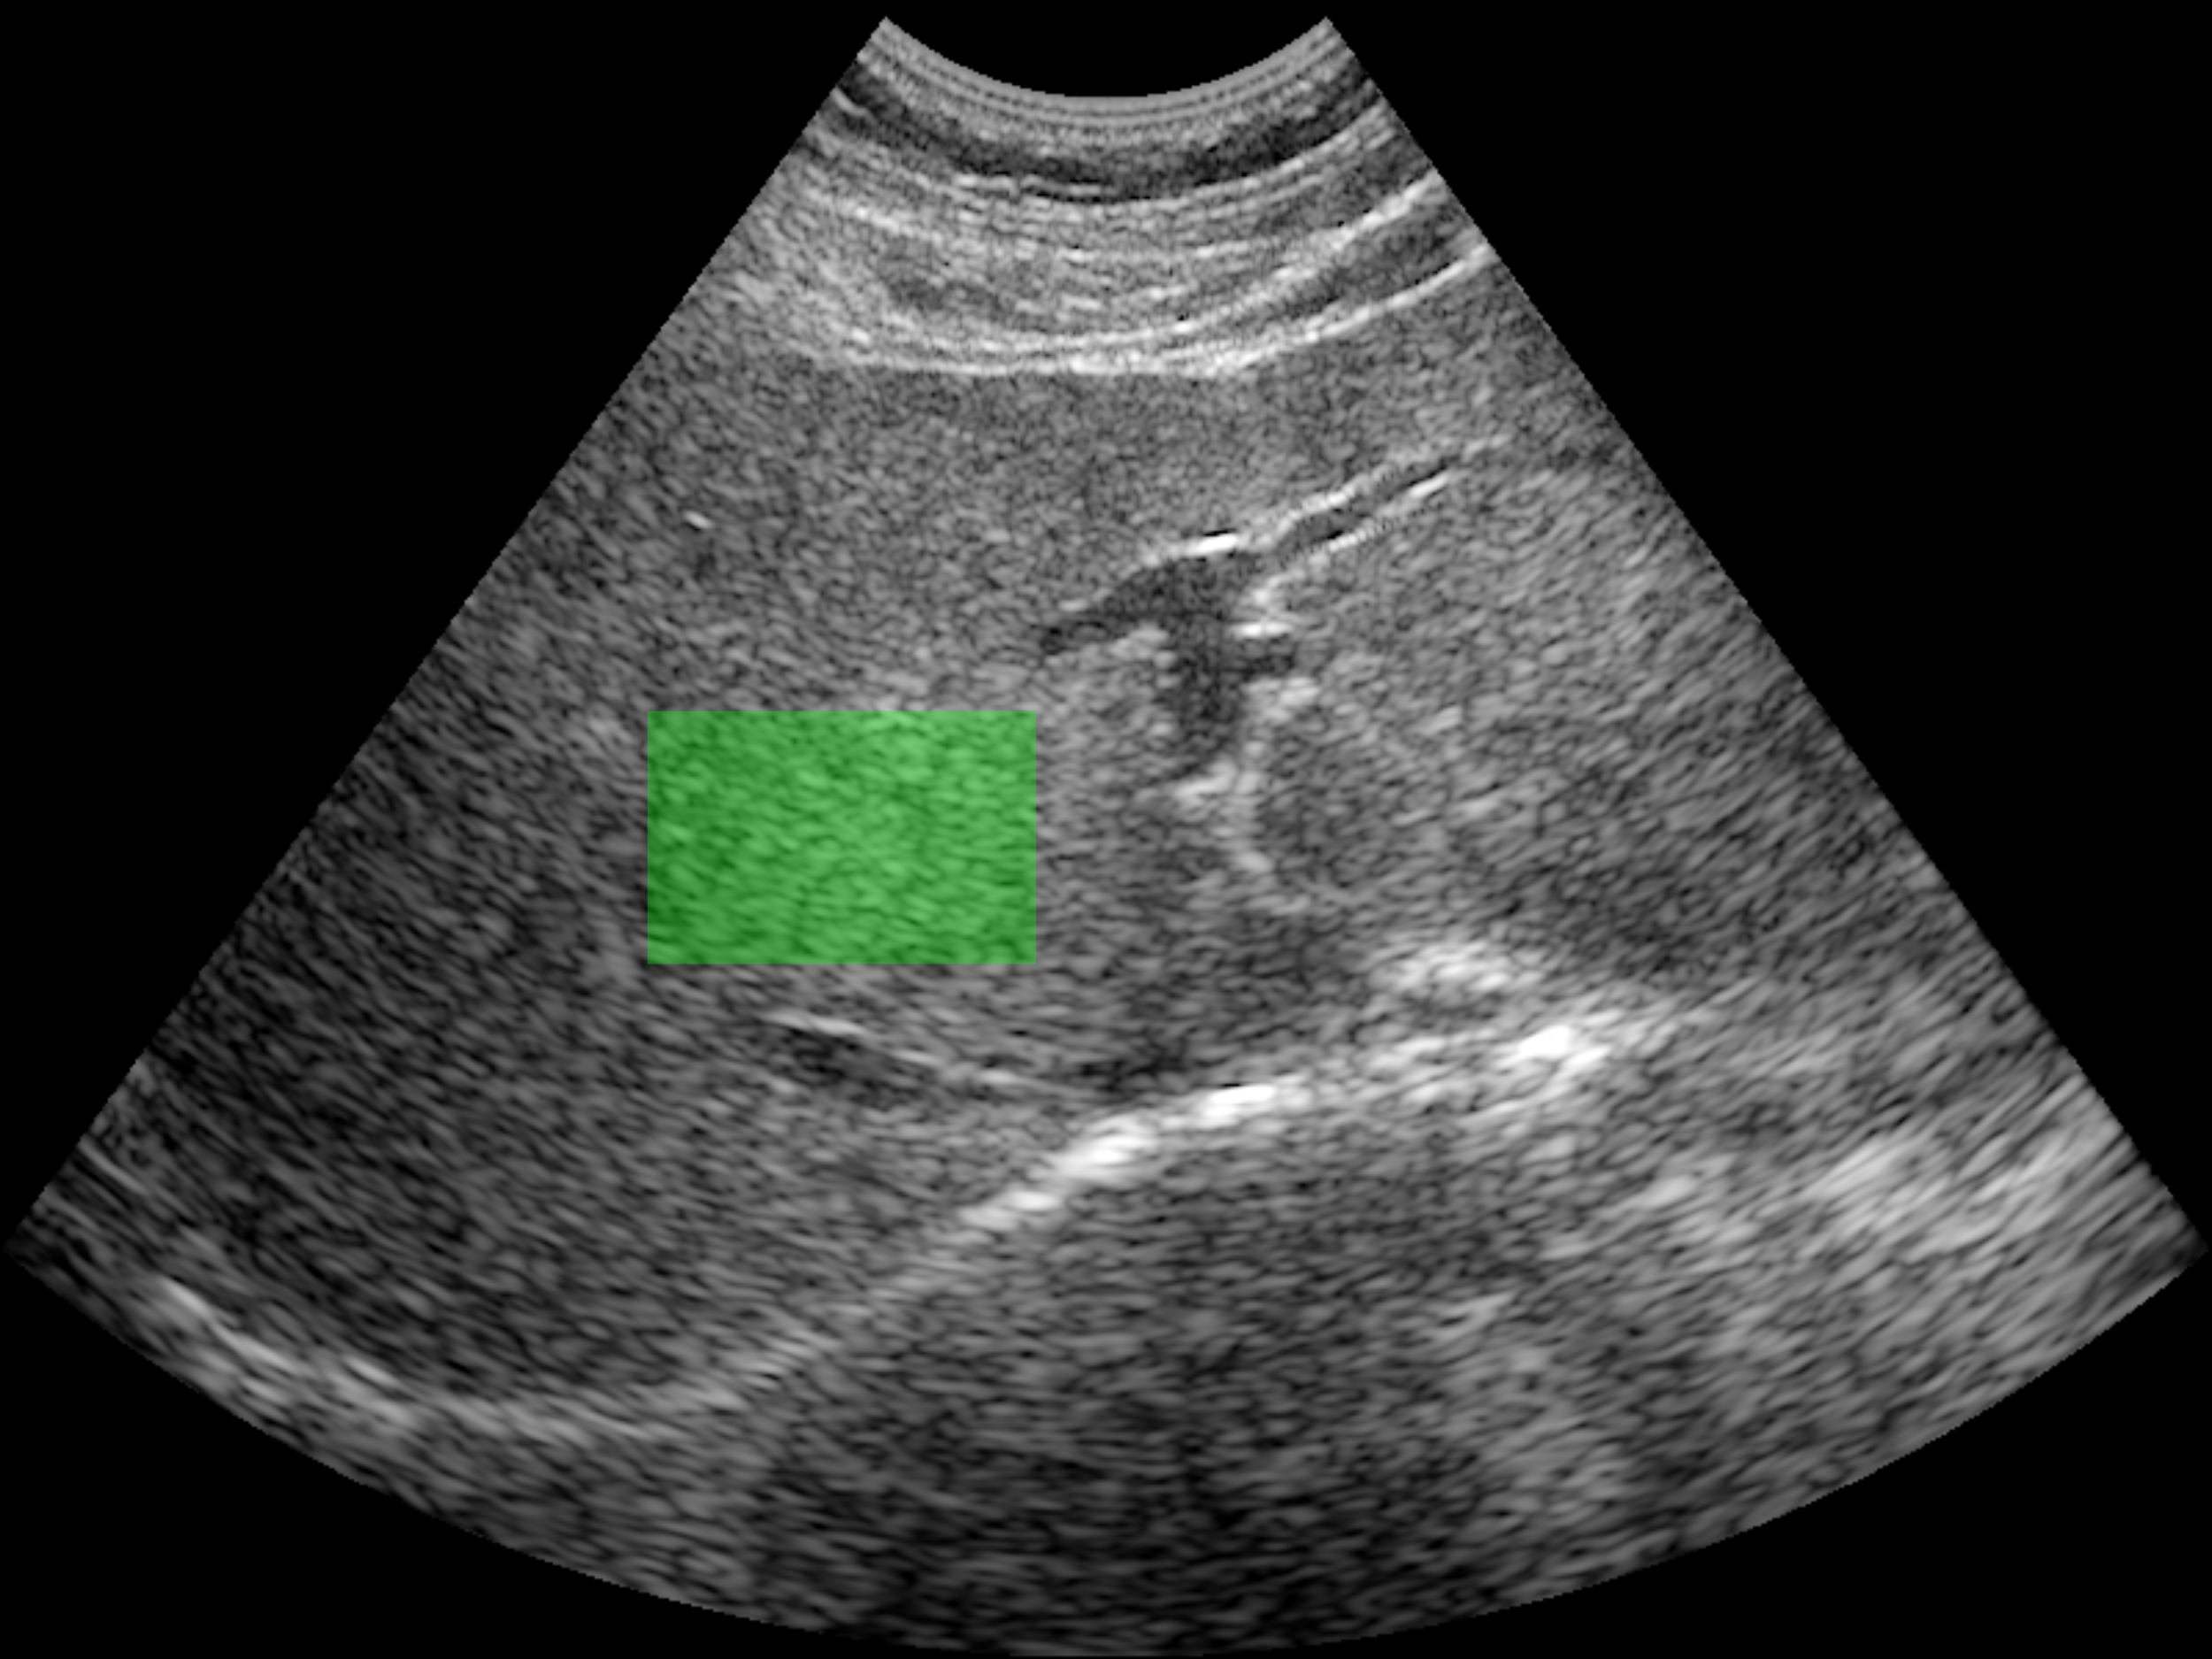
\includegraphics[width=\textwidth]{figures/liver_roi.png}
  \end{minipage}
  \begin{minipage}[c]{0.215\textwidth}
    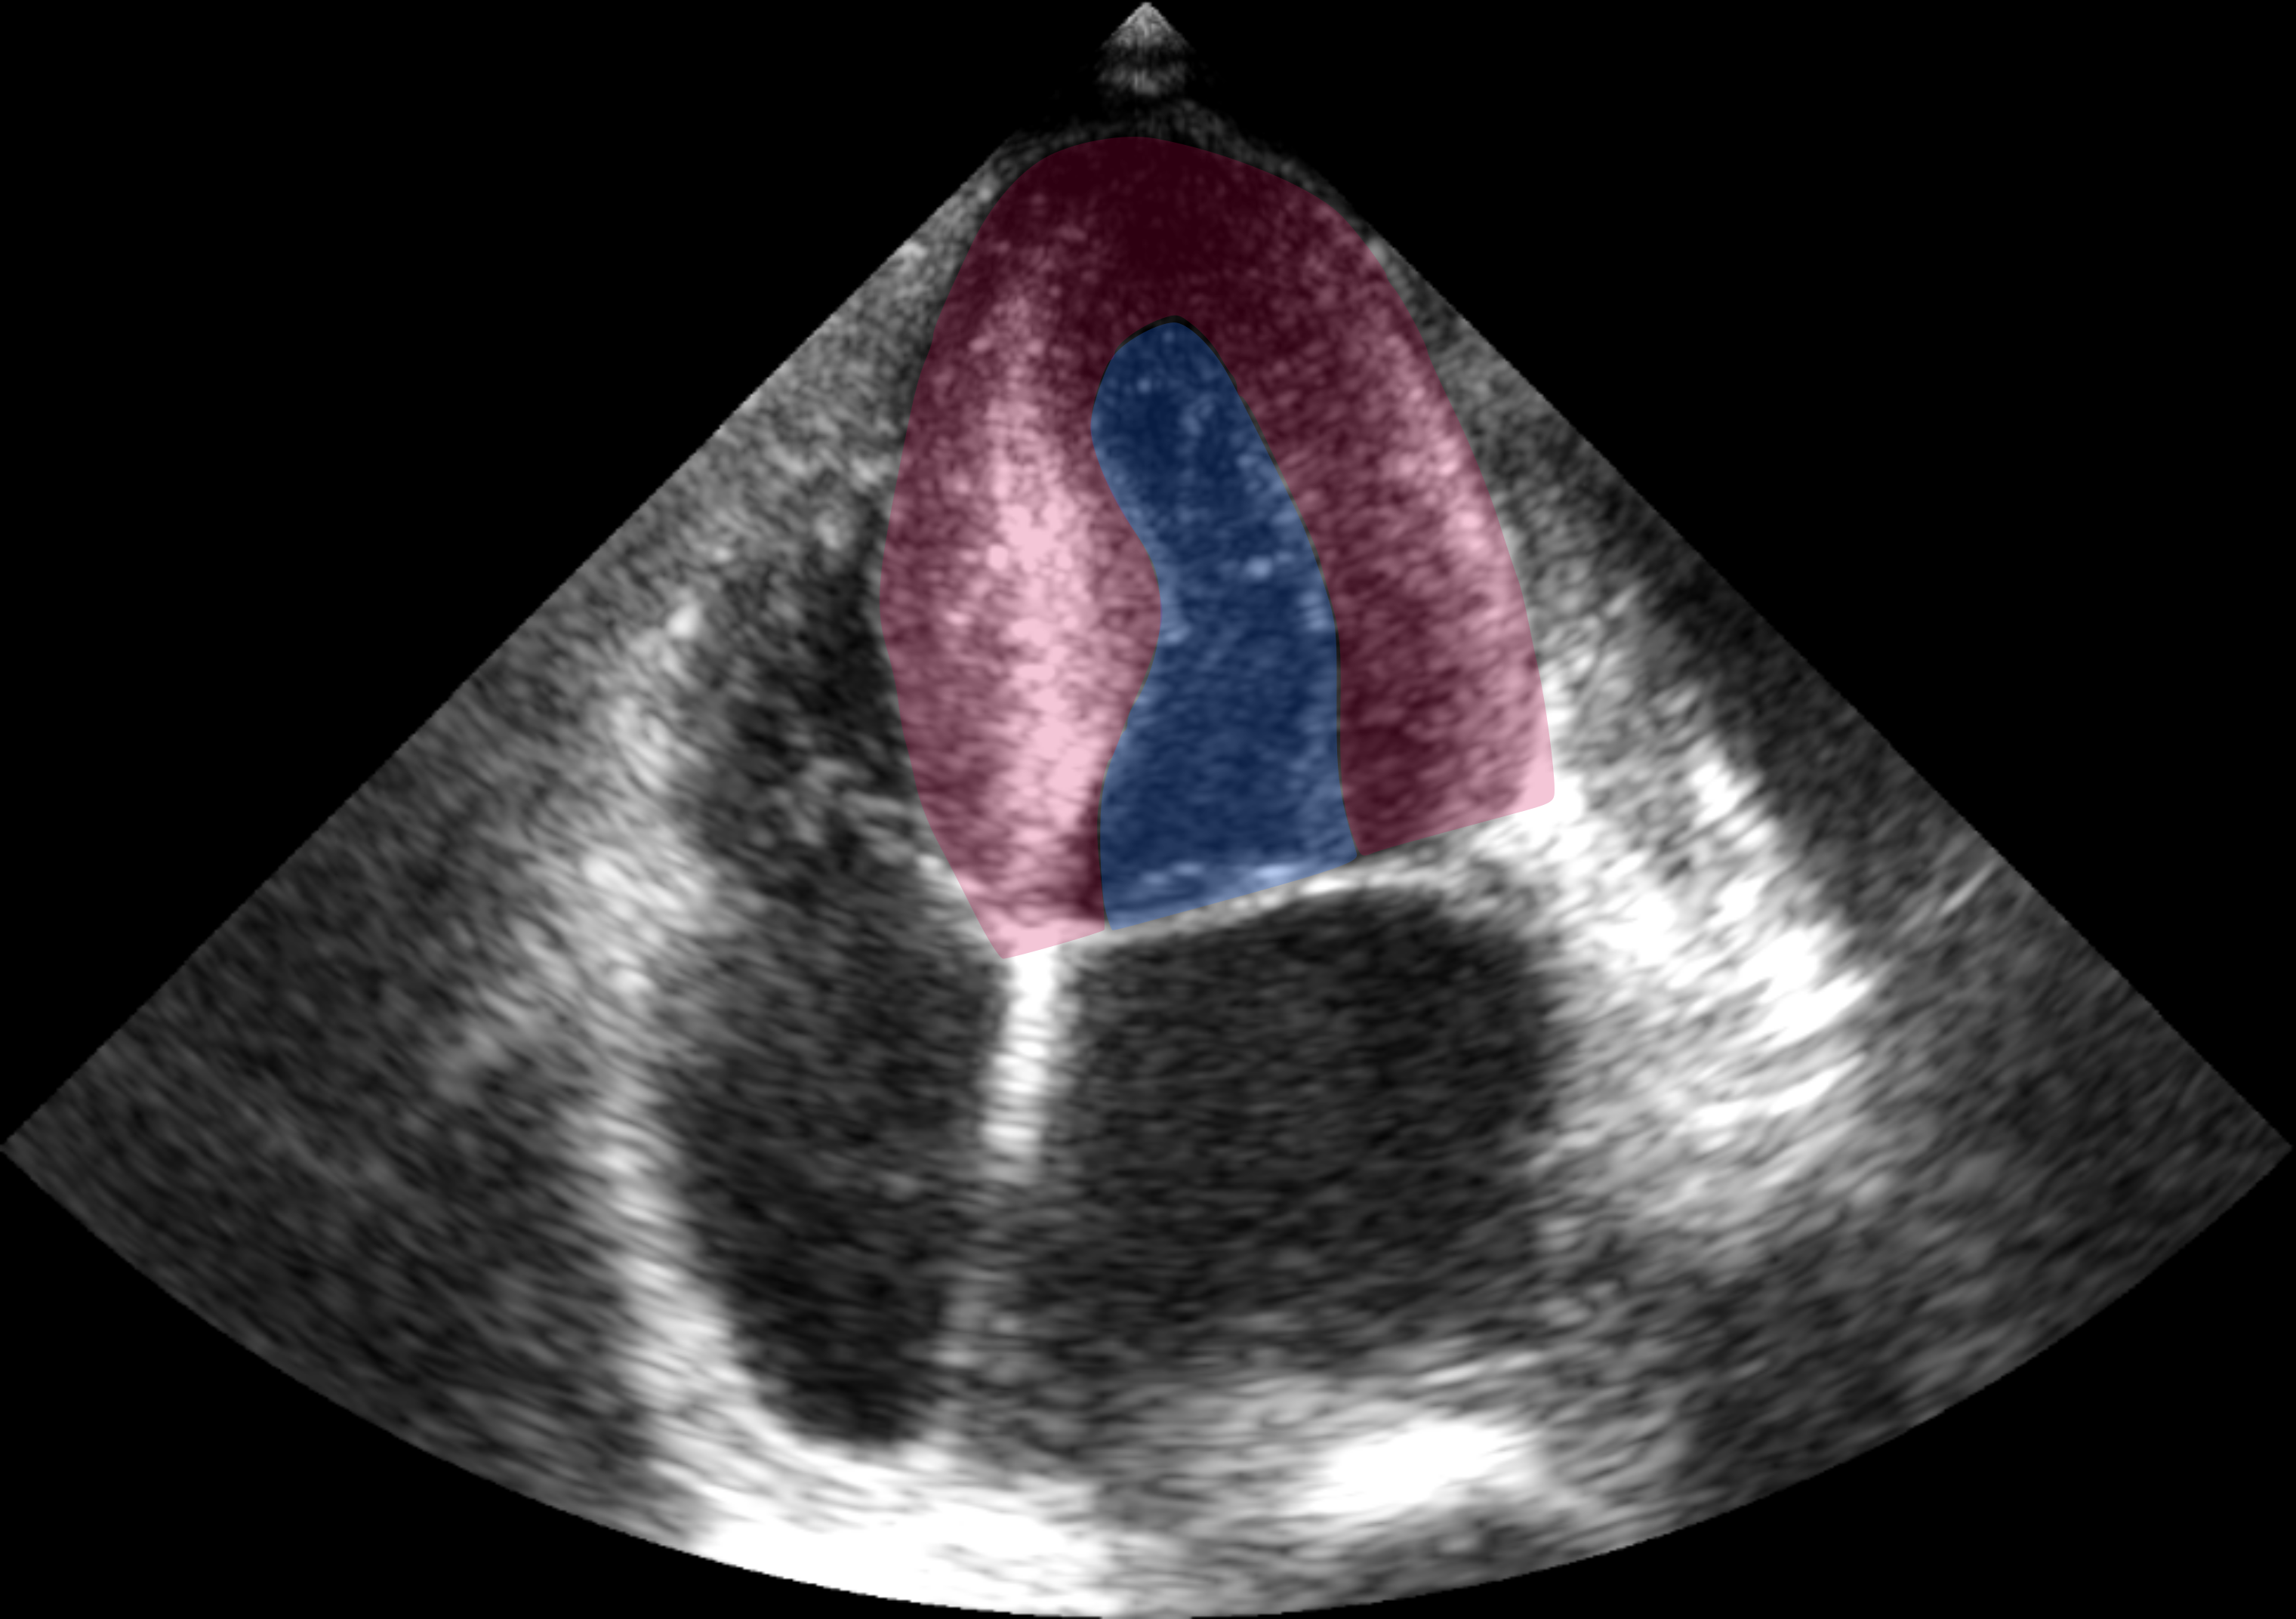
\includegraphics[width=\textwidth]{figures/cardiac_roi.png}
  \end{minipage}
  \caption{}
\end{figure}

\subsection{Phantom Experiment}
\subsection{\textit{in vivo} Experiment}

\begin{table*}
  \centering
  \caption{Objective Performance Comparison on a Liver}
  \begin{threeparttable}
  \begin{tabular}{llrrr}
    \toprule
    & \multicolumn{1}{c}{\textbf{Algorithm}}
    & \multicolumn{1}{c}{\textbf{SSNR} \texttt{[dB]}}
    & \multicolumn{1}{c}{\textbf{SSIM}}
    & \multicolumn{1}{c}{\(\mathbf{S_{3}}\)} \\\midrule
    \multirow{6}{*}{Baselines} & OSRAD & \textbf{20.8 (20.3, 21.2)} & 0.792 (0.791, 0.794) & 0.476 (0.473, 0.481)\\
    & ADMSS & 16.9 (16.5, 17.4) & \textbf{0.927 (0.893, 0.963)} & 0.350 (0.347, 0.353) \\
    & LPNDSF & 19.7 (19.4, 20.0) & 0.763 (0.762, 0.764)         & 0.343 (0.340, 0.346) \\
    & MNLM & \textbf{22.1 (21.6, 22.7)} & 0.811 (0.809, 0.812)  & 0.033 (0.329, 0.342) \\
    & NLLR & \textbf{22.0 (21.6, 22.5)} & 0.764 (0.762, 0.765)  & 0.141 (0.140, 0.142) \\
    & PFDTV & \textbf{20.0 (19.6, 20.4)} & 0.822 (0.820, 0.823) & 0.461 (0.456, 0.465) \\
    \midrule
    \multirow{5}{*}{This work} & CLPD-obj.  & \textbf{21.0 (20.7, 21.4)} & \textbf{0.914 (0.913, 0.914)} & \textbf{0.509 (0.507, 0.511)} \\
    & CLPD-A  & 19.9 (19.6, 20.2) & 0.883 (0.882, 0.884) & \textbf{0.490 (0.486, 0.494)} \\
    & CLPD-B  & 19.8 (19.6, 20.2) & \textbf{0.913 (0.913, 0.914)} & \textbf{0.507 (0.503, 0.511)} \\
    & CLPD-C  & 18.2 (18.0, 18.5) & \textbf{0.954 (0.953, 0.954)} & \textbf{0.587 (0.581, 0.592)} \\
    & CLPD-D & 19.0 (18.7, 19.3) & \textbf{0.933 (0.932, 0.933)} &  \textbf{0.565 (0.562, 0.569)} \\\bottomrule
  \end{tabular}
  \begin{tablenotes}
    \item[*] We report the average, 10\%, and \%90 percentiles of the metrics taken over 16 frames.
    \item[*] The performance of the top 5 algorithms for each metric are shown in bold face.
  \end{tablenotes}
  \end{threeparttable}
\end{table*}

\begin{table*}
  \centering
  \caption{Objective Performance Comparison on a Liver}
  \begin{threeparttable}
  \begin{tabular}{llrrrrr}
    \toprule
    & \multicolumn{1}{c}{\textbf{Algorithm}}
    & \multicolumn{1}{c}{\textbf{gCNR}}
    & \multicolumn{1}{c}{\textbf{CNR} \texttt{[dB]}}
    & \multicolumn{1}{c}{\textbf{SSNR} \texttt{[dB]}}
    & \multicolumn{1}{c}{\textbf{SSIM}}
    & \multicolumn{1}{c}{\(\mathbf{S_{3}}\)} \\\midrule
    \multirow{6}{*}{Baselines}
    & OSRAD  & 0.490          & -1.62          & 4.51          & 0.891          & 0.500 \\
    & ADMSS  & 0.467          & -1.67          & 4.33          & \textbf{0.967} & 0.204 \\
    & LPNDSF & 0.473          & -1.67          & 4.39          & 0.868          & 0.458 \\
    & MNLM   & \textbf{0.534} & \textbf{-1.61} & 4.42          & 0.918          & 0.414 \\
    & NLLR   & \textbf{0.501} & \textbf{-1.60} & 4.61          & 0.857          & 0.042\\
    & PFDTV  & 0.480          & -1.65          & 4.49          & 0.865          & 0.155 \\\midrule
    \multirow{4}{*}{This work}
    & CLPD-A & 0.484          & -1.64          & \textbf{4.64} & \textbf{0.957} & \textbf{0.858} \\
    & CLPD-B & \textbf{0.496} & \textbf{-1.55} & \textbf{4.69} & \textbf{0.949} & \textbf{0.685} \\
    & CLPD-E & 0.476          & -1.63          & \textbf{4.61} & \textbf{0.961} & \textbf{0.507} \\
    & CLPD-F & \textbf{0.507} & \textbf{-1.50} & \textbf{4.79} & 0.920          & \textbf{0.705} \\\bottomrule
  \end{tabular}
  \begin{tablenotes}
    \item[*] The performance of the top 4 algorithms for each metric are shown in bold face.
  \end{tablenotes}
  \end{threeparttable}
\end{table*}


\begin{figure*}
  \centering
  \begin{subfigure}[b]{0.15\textwidth}
    \begin{tikzpicture}[
        spy using outlines={%
          rectangle,magnification=3,size=\textwidth,
          every spy on node/.append style={transparentwindow}
        }
      ]
      \node (figA) at (0.0,0.0) {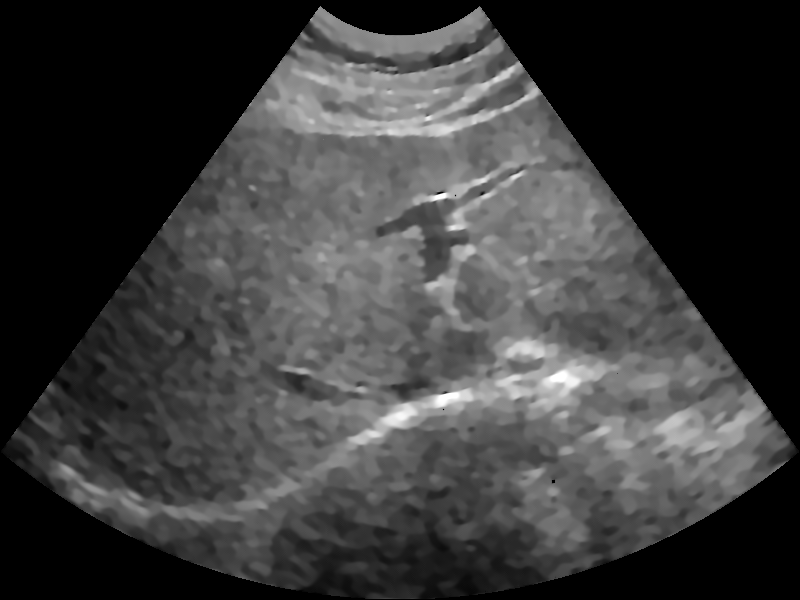
\includegraphics[width=\textwidth, trim={4cm 4cm 4cm 0cm}, clip]{figures/liver1_osrad.png}};
      \spy on (0.15, 0.0) in node [redwindow, anchor=north] at ($(figA.south)$);
    \end{tikzpicture}
    \caption{OSRAD}\label{fig:liver1_osrad}
  \end{subfigure}%
  \begin{subfigure}[b]{0.15\textwidth}
    \begin{tikzpicture}[
        spy using outlines={%
          rectangle, magnification=3,size=\textwidth,
          every spy on node/.append style={transparentwindow}
        }
      ]
      \node (figA) at (0.0,0.0) {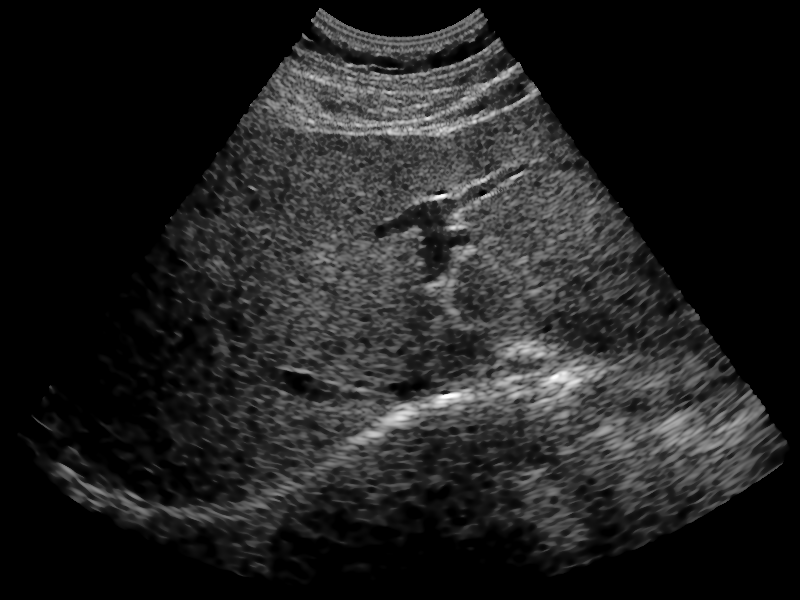
\includegraphics[width=\textwidth, trim={4cm 4cm 4cm 0cm}, clip]{figures/liver1_admss.png}};
      \spy on (0.15, 0.0) in node [redwindow, anchor=north] at ($(figA.south)$);
    \end{tikzpicture}
    \caption{ADMSS}\label{fig:liver1_admss}
  \end{subfigure}%
  \begin{subfigure}[b]{0.15\textwidth}
    \begin{tikzpicture}[
        spy using outlines={%
          rectangle, magnification=3,size=\textwidth,
          every spy on node/.append style={transparentwindow}
        }
      ]
      \node (figA) at (0.0,0.0) {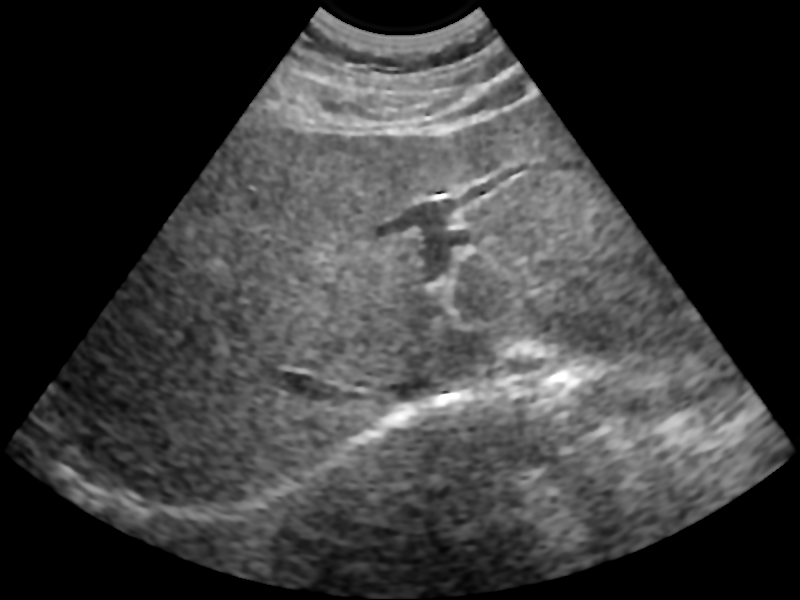
\includegraphics[width=\textwidth, trim={4cm 4cm 4cm 0cm}, clip]{figures/liver1_lpndsf.png}};
      \spy on (0.15, 0.0) in node [redwindow, anchor=north] at ($(figA.south)$);
    \end{tikzpicture}
    \caption{LPNDSF}\label{fig:liver1_lpndsf}
  \end{subfigure}%
  \begin{subfigure}[b]{0.15\textwidth}
    \begin{tikzpicture}[
        spy using outlines={%
          rectangle,magnification=3,size=\textwidth,
          every spy on node/.append style={transparentwindow}
        }
      ]
      \node (figA) at (0.0,0.0) {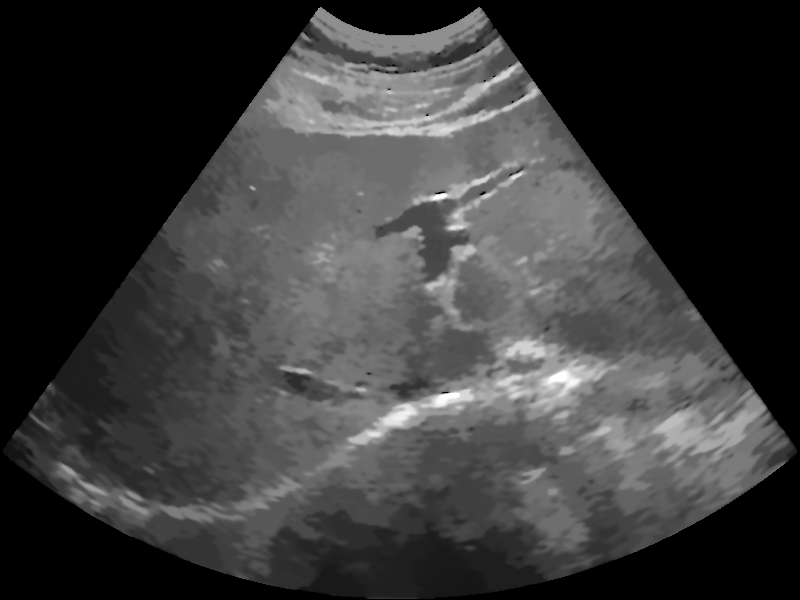
\includegraphics[width=\textwidth, trim={4cm 4cm 4cm 0cm}, clip]{figures/liver1_mnlm.png}};
      \spy on (0.15, 0.0) in node [redwindow, anchor=north] at ($(figA.south)$);
    \end{tikzpicture}
    \caption{MNLM}\label{fig:liver1_mnlm}
  \end{subfigure}%
  \begin{subfigure}[b]{0.15\textwidth}
    \begin{tikzpicture}[
        spy using outlines={%
          rectangle,magnification=3,size=\textwidth,
          every spy on node/.append style={transparentwindow}
        }
      ]
      \node (figA) at (0.0,0.0) {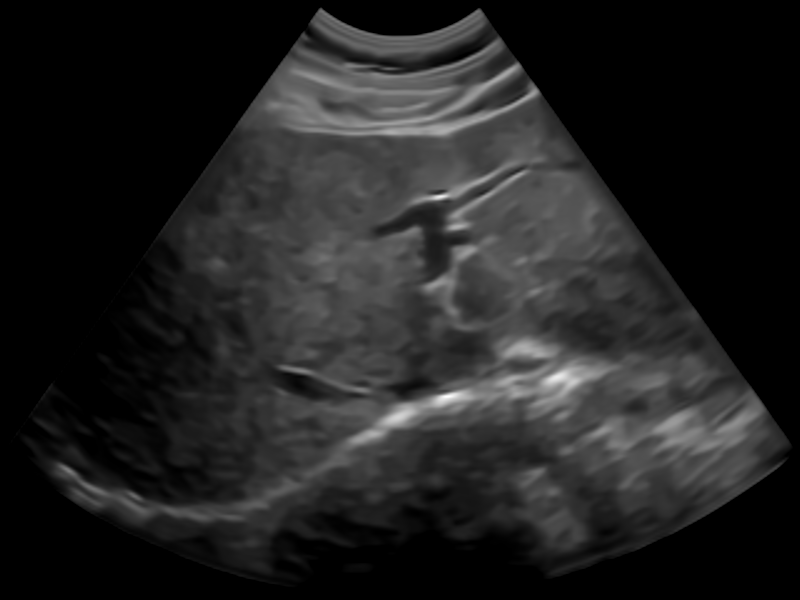
\includegraphics[width=\textwidth, trim={4cm 4cm 4cm 0cm}, clip]{figures/liver1_nllr.png}};
      \spy on (0.15, 0.0) in node [redwindow, anchor=north] at ($(figA.south)$);
    \end{tikzpicture}
    \caption{NLLR}\label{fig:liver1_nllr}
  \end{subfigure}%
  \begin{subfigure}[b]{0.15\textwidth}
    \begin{tikzpicture}[
        spy using outlines={%
          rectangle,magnification=3,size=\textwidth,
          every spy on node/.append style={transparentwindow}
        }
      ]
      \node (figA) at (0.0,0.0) {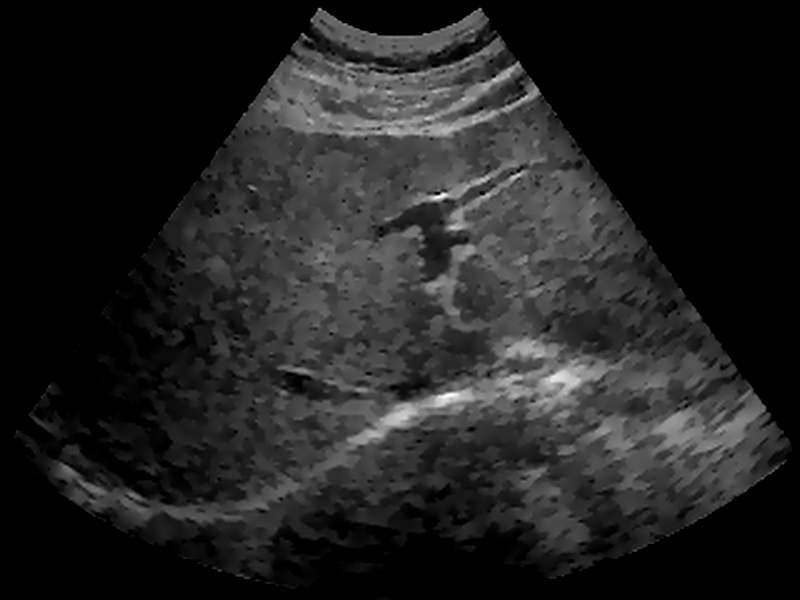
\includegraphics[width=\textwidth, trim={4cm 4cm 4cm 0cm}, clip]{figures/liver1_pfdtv.png}};
      \spy on (0.15, 0.0) in node [redwindow, anchor=north] at ($(figA.south)$);
    \end{tikzpicture}
    \caption{PFDTV}\label{fig:liver1_pfdtv}
  \end{subfigure}\\
  \begin{subfigure}[b]{0.15\textwidth}
    \begin{tikzpicture}[
        spy using outlines={%
          rectangle,magnification=3,size=\textwidth,
          every spy on node/.append style={transparentwindow}
        }
      ]
      \node (figA) at (0.0,0.0) {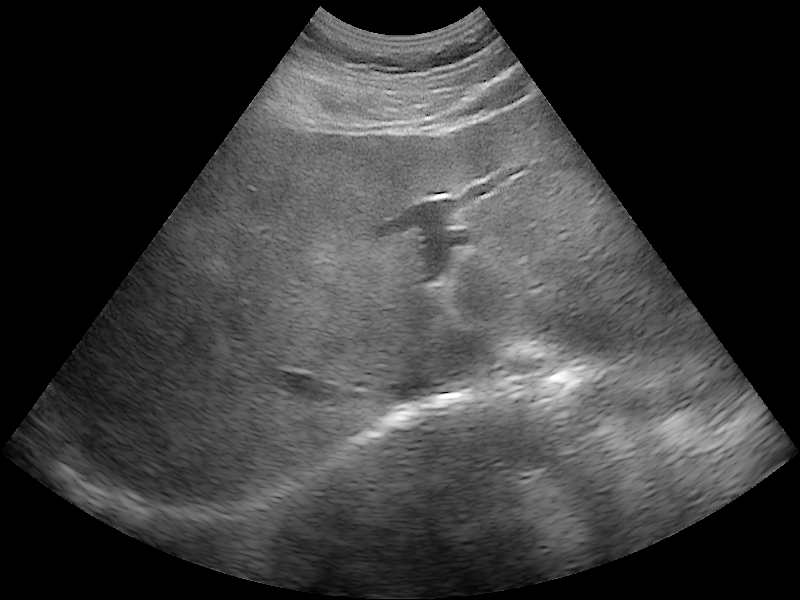
\includegraphics[width=\textwidth, trim={4cm 4cm 4cm 0cm}, clip]{figures/liver1_clpdQ.png}};
      \spy on (0.15, 0.0) in node [redwindow, anchor=north] at ($(figA.south)$);
    \end{tikzpicture}
    \caption{CLPD-SSNR}\label{fig:liver1_clpdssnr}
  \end{subfigure}%
  \begin{subfigure}[b]{0.15\textwidth}
    \begin{tikzpicture}[
        spy using outlines={%
          rectangle,magnification=3,size=\textwidth,
          every spy on node/.append style={transparentwindow}
        }
      ]
      \node (figA) at (0.0,0.0) {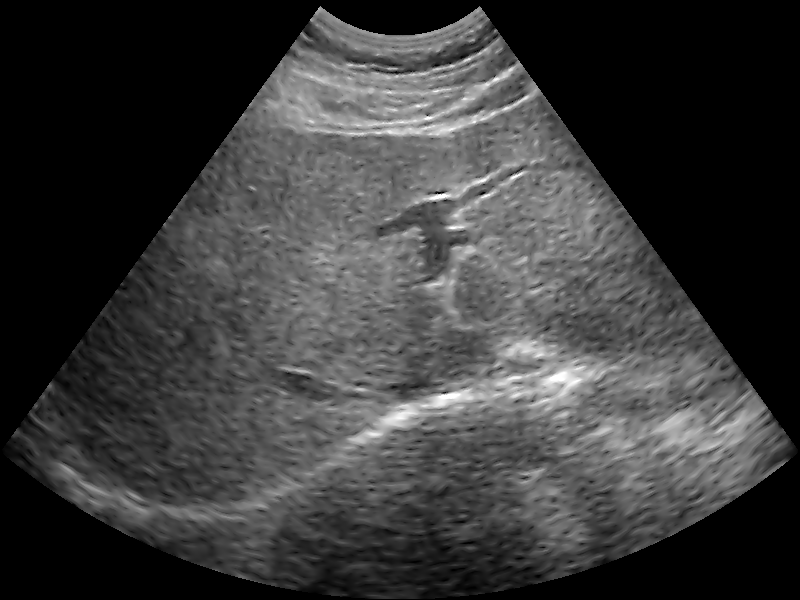
\includegraphics[width=\textwidth, trim={4cm 4cm 4cm 0cm}, clip]{figures/liver1_clpda.png}};
      \spy on (0.15, 0.0) in node [redwindow, anchor=north] at ($(figA.south)$);
    \end{tikzpicture}
    \caption{CLPD-A}\label{fig:liver1_clpda}
  \end{subfigure}%
  \begin{subfigure}[b]{0.15\textwidth}
    \begin{tikzpicture}[
        spy using outlines={%
          rectangle,magnification=3,size=\textwidth,
          every spy on node/.append style={transparentwindow}
        }
      ]
      \node (figA) at (0.0,0.0) {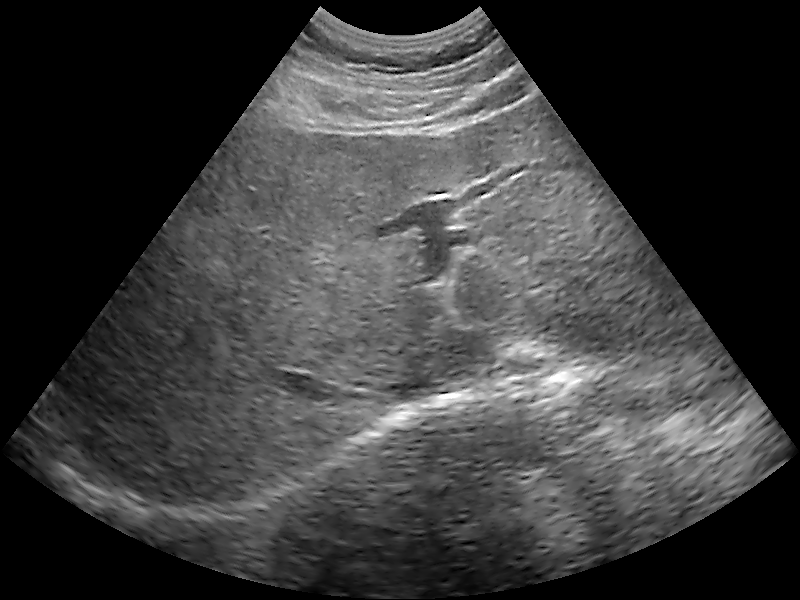
\includegraphics[width=\textwidth, trim={4cm 4cm 4cm 0cm}, clip]{figures/liver1_clpdb.png}};
      \spy on (0.15, 0.0) in node [redwindow, anchor=north] at ($(figA.south)$);
    \end{tikzpicture}
    \caption{CLPD-B}\label{fig:liver1_clpdb}
  \end{subfigure}%
  \begin{subfigure}[b]{0.15\textwidth}
    \begin{tikzpicture}[
        spy using outlines={%
          rectangle,magnification=3,size=\textwidth,
          every spy on node/.append style={transparentwindow}
        }
      ]
      \node (figA) at (0.0,0.0) {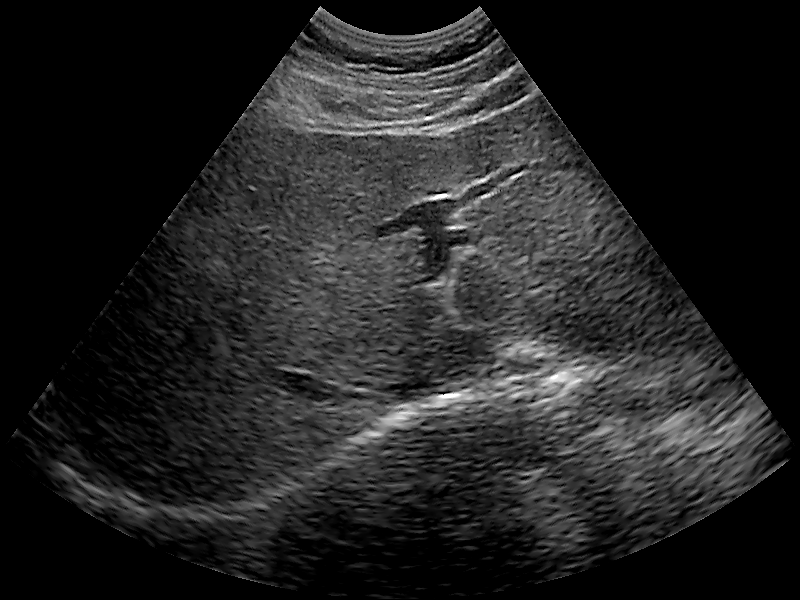
\includegraphics[width=\textwidth, trim={4cm 4cm 4cm 0cm}, clip]{figures/liver1_clpdc.png}};
      \spy on (0.15, 0.0) in node [redwindow, anchor=north] at ($(figA.south)$);
    \end{tikzpicture}
    \caption{CLPD-C}\label{fig:liver1_clpdc}
  \end{subfigure}%
  \begin{subfigure}[b]{0.15\textwidth}
    \begin{tikzpicture}[
        spy using outlines={%
          rectangle,magnification=3,size=\textwidth,
          every spy on node/.append style={transparentwindow}
        }
      ]
      \node (figA) at (0.0,0.0) {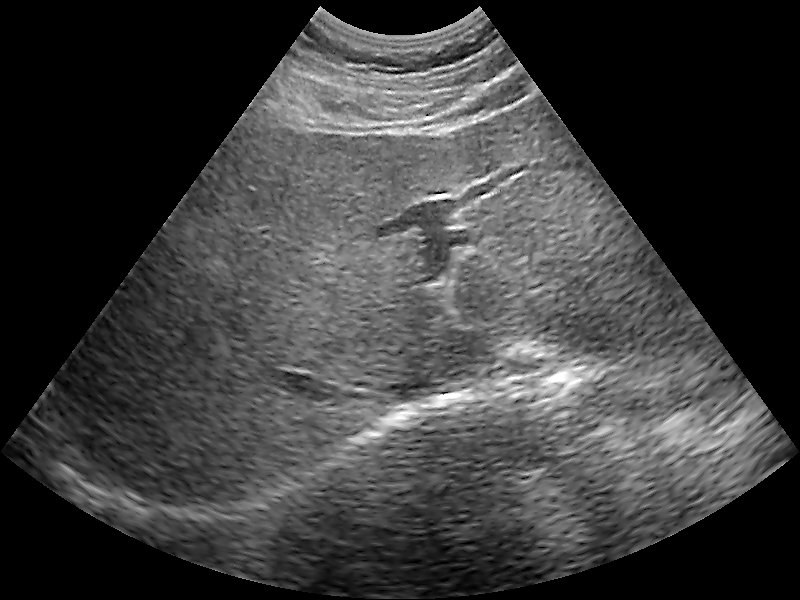
\includegraphics[width=\textwidth, trim={4cm 4cm 4cm 0cm}, clip]{figures/liver1_clpdd.png}};
      \spy on (0.15, 0.0) in node [redwindow, anchor=north] at ($(figA.south)$);
    \end{tikzpicture}
    \caption{CLPD-D}\label{fig:liver1_clpdd}
  \end{subfigure}%
  \begin{subfigure}[b]{0.15\textwidth}
    \begin{tikzpicture}[
        spy using outlines={%
          rectangle,magnification=3,size=\textwidth,
          every spy on node/.append style={redwindow}
        }
      ]
      \node (figA) at (0.0,0.0) {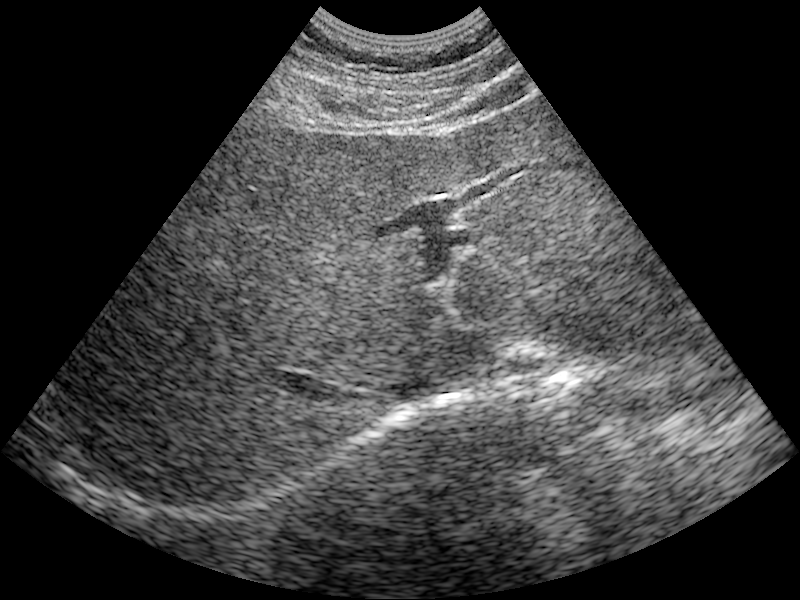
\includegraphics[width=\textwidth, trim={4cm 4cm 4cm 0cm}, clip]{figures/liver1.png}};
      \spy on (0.15, 0.0) in node [redwindow, anchor=north] at ($(figA.south)$);
    \end{tikzpicture}
    \caption{Original}\label{fig:liver_original}
  \end{subfigure}
  \caption{Results on a liver subcostal-view image.}\label{fig:liver1}
\end{figure*}

%%% Local Variables:
%%% TeX-master: "master"
%%% End:


\begin{figure*}
  \vspace{-0.2in}
  \centering
  \begin{subfigure}[b]{0.15\textwidth}
    \begin{tikzpicture}[
        spy using outlines={%
          rectangle,magnification=3,size=\textwidth,
          every spy on node/.append style={transparentwindow}
        }
      ]
      \node (figA) at (0.0,0.0) {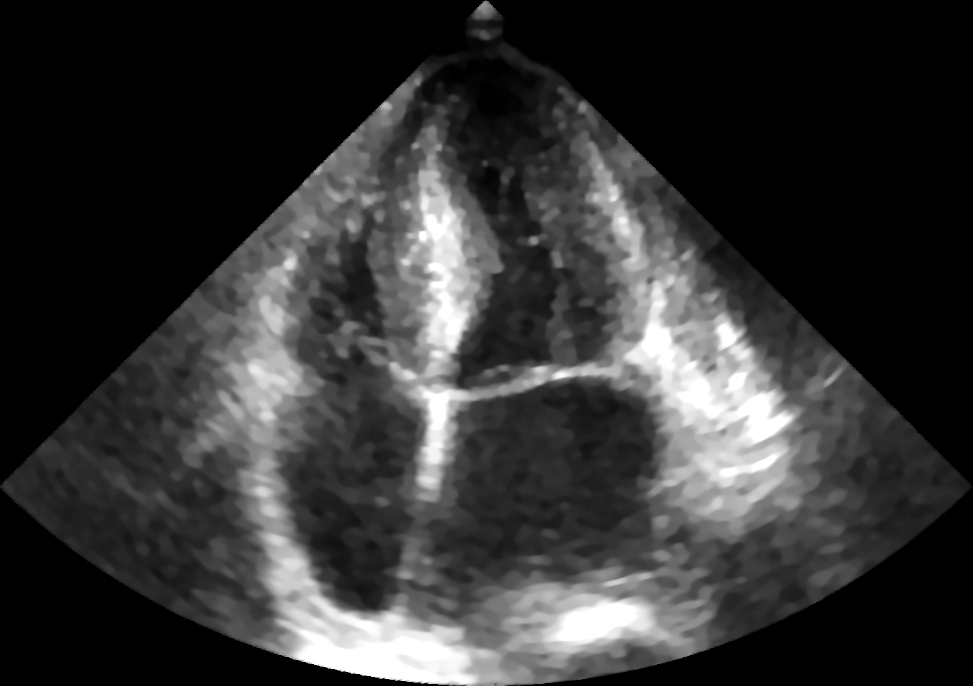
\includegraphics[width=\textwidth]{figures/cardiac3_osrad.png}};
      \spy on (0.1, 0.2) in node [redwindow, anchor=north] at ($(figA.south)$);
    \end{tikzpicture}
    \caption{OSRAD}
  \end{subfigure}%
  \begin{subfigure}[b]{0.15\textwidth}
    \begin{tikzpicture}[
        spy using outlines={%
          rectangle, magnification=3,size=\textwidth,
          every spy on node/.append style={transparentwindow}
        }
      ]
      \node (figA) at (0.0,0.0) {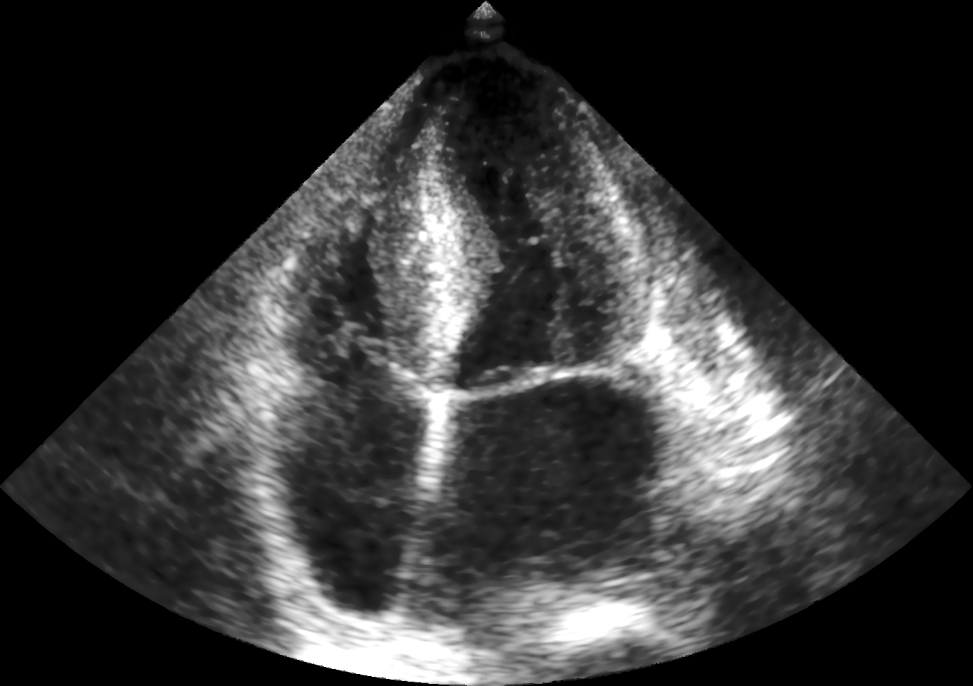
\includegraphics[width=\textwidth]{figures/cardiac3_admss.png}};
      \spy on (0.1, 0.2) in node [redwindow, anchor=north] at ($(figA.south)$);
    \end{tikzpicture}
    \caption{ADMSS}
  \end{subfigure}%
  \begin{subfigure}[b]{0.15\textwidth}
    \begin{tikzpicture}[
        spy using outlines={%
          rectangle, magnification=3,size=\textwidth,
          every spy on node/.append style={transparentwindow}
        }
      ]
      \node (figA) at (0.0,0.0) {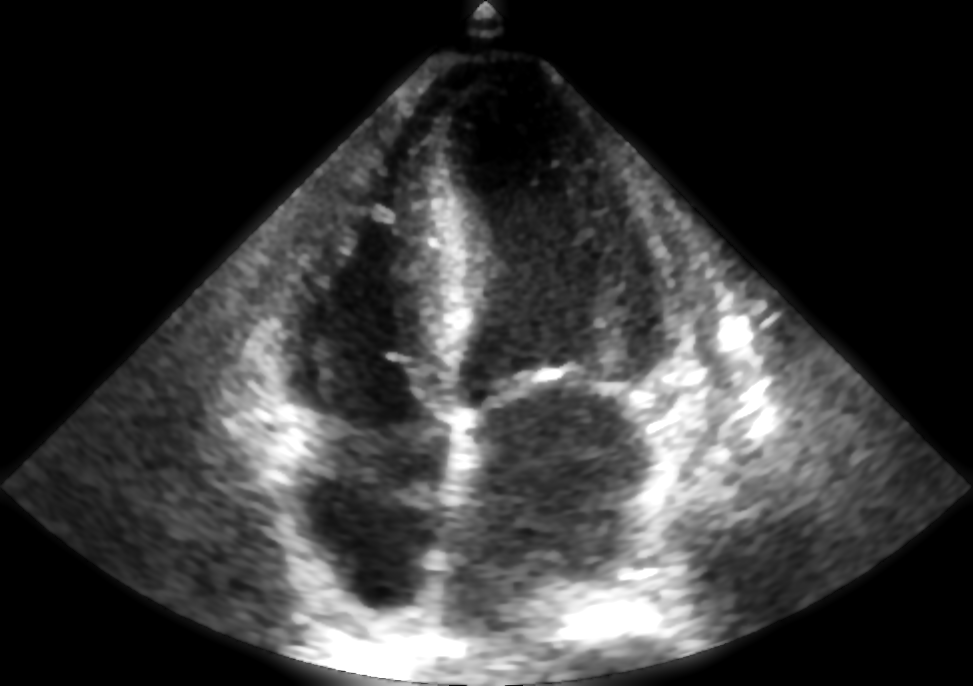
\includegraphics[width=\textwidth]{figures/cardiac3_lpndsf.png}};
      \spy on (0.1, 0.2) in node [redwindow, anchor=north] at ($(figA.south)$);
    \end{tikzpicture}
    \caption{LPNDSF}
  \end{subfigure}%
  \begin{subfigure}[b]{0.15\textwidth}
    \begin{tikzpicture}[
        spy using outlines={%
          rectangle,magnification=3,size=\textwidth,
          every spy on node/.append style={transparentwindow}
        }
      ]
      \node (figA) at (0.0,0.0) {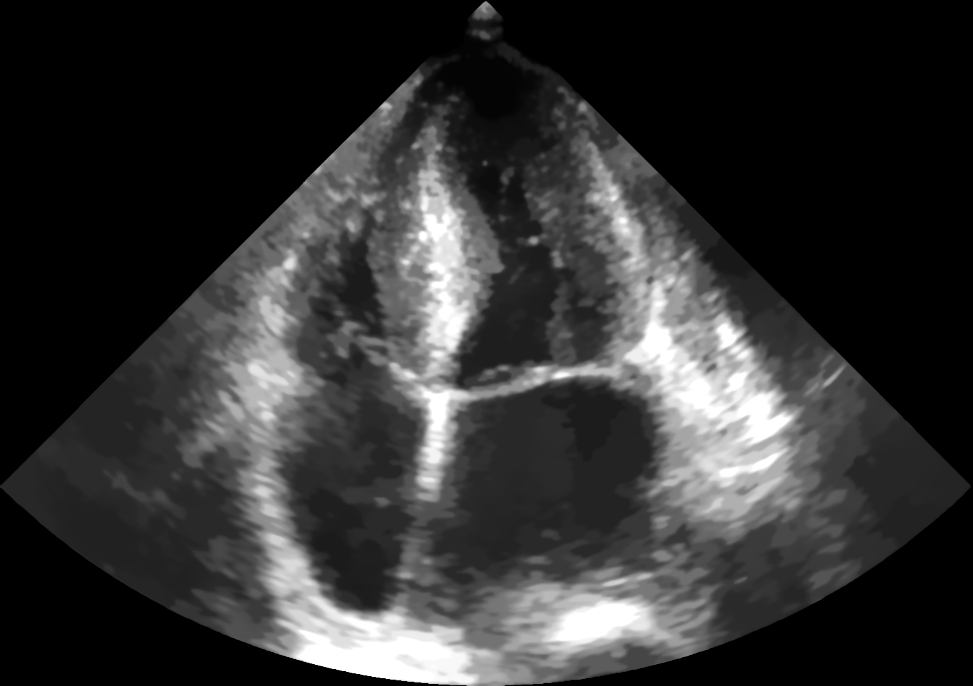
\includegraphics[width=\textwidth]{figures/cardiac3_mnlm.png}};
      \spy on (0.1, 0.2) in node [redwindow, anchor=north] at ($(figA.south)$);
    \end{tikzpicture}
    \caption{MNLM}
  \end{subfigure}%
  \begin{subfigure}[b]{0.15\textwidth}
    \begin{tikzpicture}[
        spy using outlines={%
          rectangle,magnification=3,size=\textwidth,
          every spy on node/.append style={transparentwindow}
        }
      ]
      \node (figA) at (0.0,0.0) {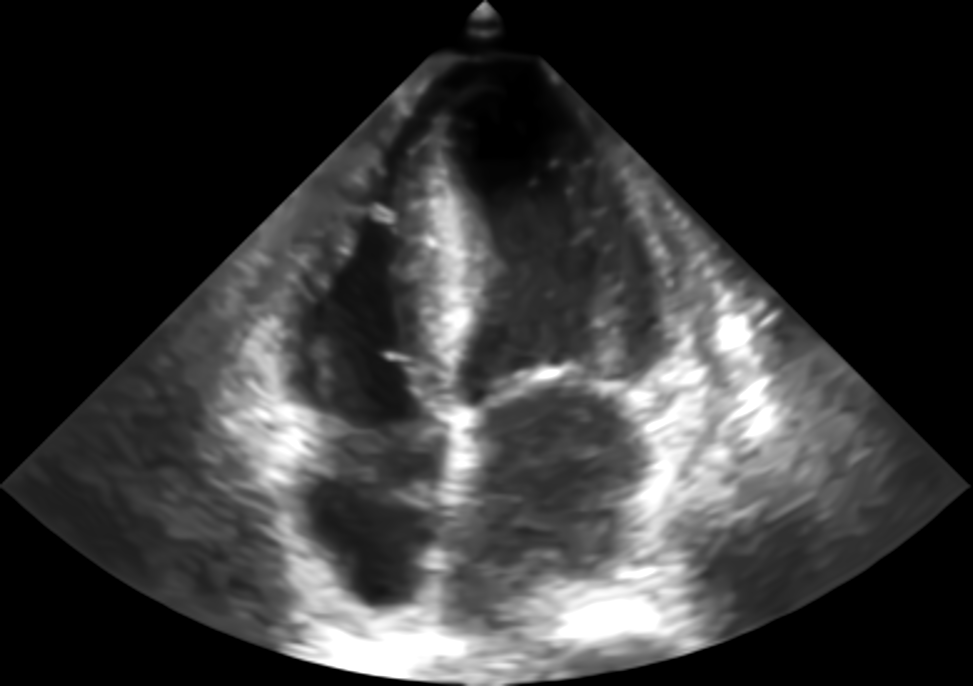
\includegraphics[width=\textwidth]{figures/cardiac3_nllr.png}};
      \spy on (0.1, 0.2) in node [redwindow, anchor=north] at ($(figA.south)$);
    \end{tikzpicture}
    \caption{NLLR}
  \end{subfigure}%
  \begin{subfigure}[b]{0.15\textwidth}
    \begin{tikzpicture}[
        spy using outlines={%
          rectangle,magnification=3,size=\textwidth,
          every spy on node/.append style={transparentwindow}
        }
      ]
      \node (figA) at (0.0,0.0) {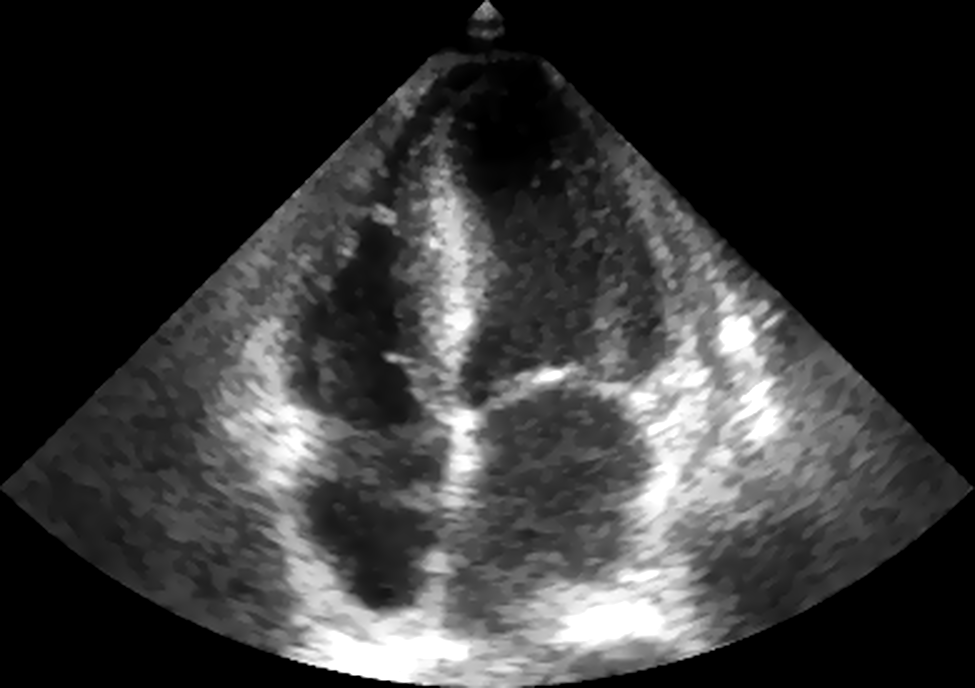
\includegraphics[width=\textwidth]{figures/cardiac3_pfdtv.png}};
      \spy on (0.1, 0.2) in node [redwindow, anchor=north] at ($(figA.south)$);
    \end{tikzpicture}
    \caption{PFDTV}
  \end{subfigure}\\
  %% \begin{subfigure}[b]{0.15\textwidth}
  %%   \begin{tikzpicture}[
  %%       spy using outlines={%
  %%         rectangle,magnification=3,size=\textwidth,
  %%         every spy on node/.append style={transparentwindow}
  %%       }
  %%     ]
  %%     \node (figA) at (0.0,0.0) {\includegraphics[width=\textwidth, trim={4cm 4cm 4cm 0cm}, clip]{figures/cardiac3_clpdQ.png}};
  %%     \spy on (0.1, 0.2) in node [redwindow, anchor=north] at ($(figA.south)$);
  %%   \end{tikzpicture}
  %%   \caption{CLPD-SSNR}
  %% \end{subfigure}%
  \begin{subfigure}[b]{0.15\textwidth}
    \begin{tikzpicture}[
        spy using outlines={%
          rectangle,magnification=3,size=\textwidth,
          every spy on node/.append style={transparentwindow}
        }
      ]
      \node (figA) at (0.0,0.0) {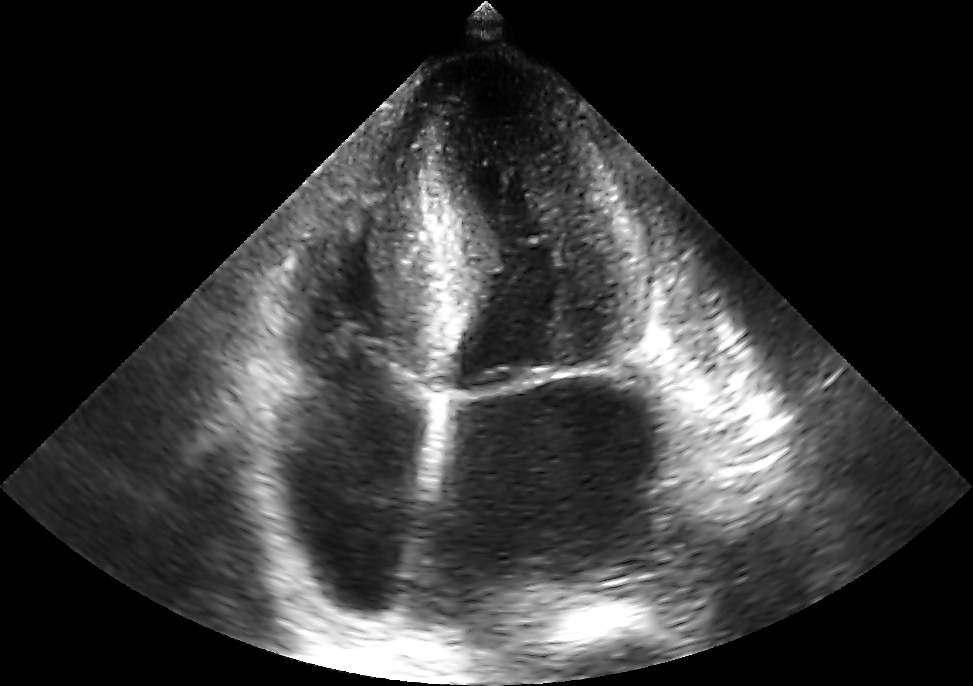
\includegraphics[width=\textwidth]{figures/cardiac3_clpda.png}};
      \spy on (0.1, 0.2) in node [redwindow, anchor=north] at ($(figA.south)$);
    \end{tikzpicture}
    \caption{CLPD-A}
  \end{subfigure}%
  \begin{subfigure}[b]{0.15\textwidth}
    \begin{tikzpicture}[
        spy using outlines={%
          rectangle,magnification=3,size=\textwidth,
          every spy on node/.append style={transparentwindow}
        }
      ]
      \node (figA) at (0.0,0.0) {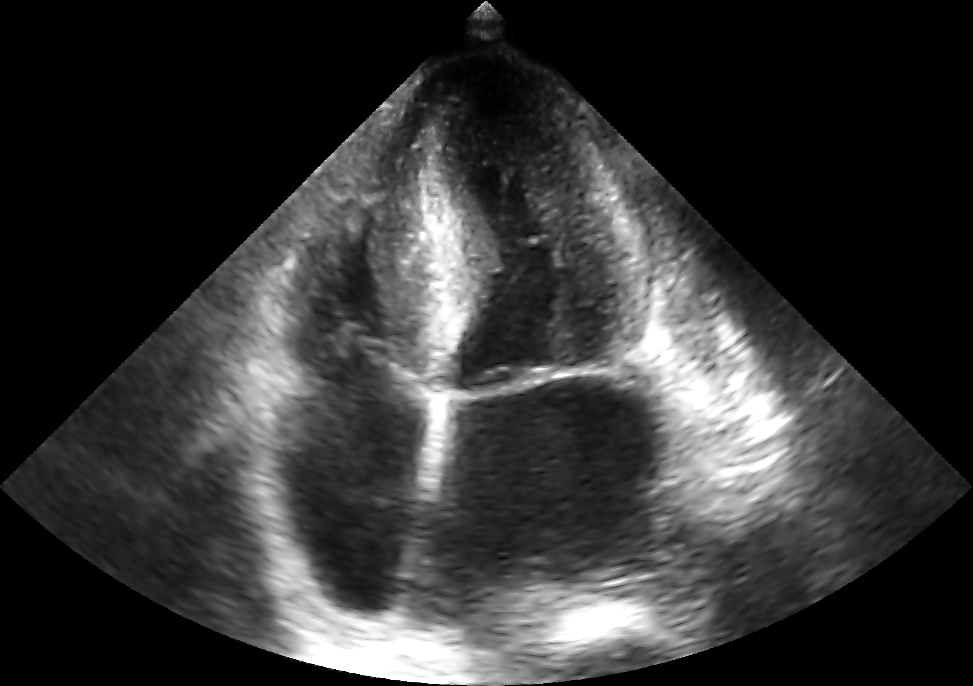
\includegraphics[width=\textwidth]{figures/cardiac3_clpdb.png}};
      \spy on (0.1, 0.2) in node [redwindow, anchor=north] at ($(figA.south)$);
    \end{tikzpicture}
    \caption{CLPD-B}
  \end{subfigure}%
  \begin{subfigure}[b]{0.15\textwidth}
    \begin{tikzpicture}[
        spy using outlines={%
          rectangle,magnification=3,size=\textwidth,
          every spy on node/.append style={transparentwindow}
        }
      ]
      \node (figA) at (0.0,0.0) {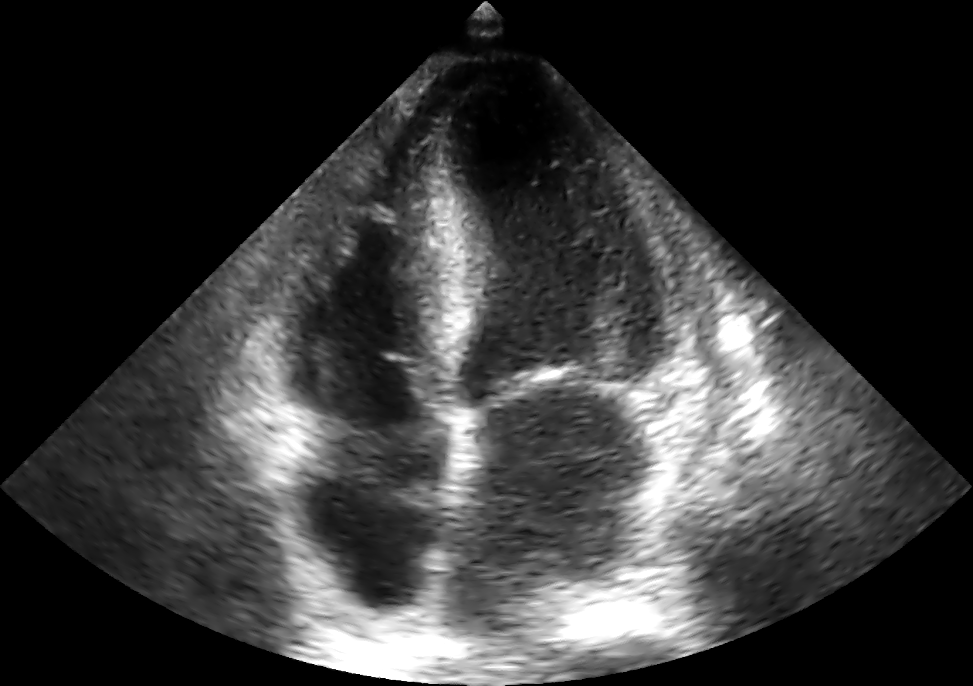
\includegraphics[width=\textwidth]{figures/cardiac3_clpde.png}};
      \spy on (0.1, 0.2) in node [redwindow, anchor=north] at ($(figA.south)$);
    \end{tikzpicture}
    \caption{CLPD-E}
  \end{subfigure}%
  \begin{subfigure}[b]{0.15\textwidth}
    \begin{tikzpicture}[
        spy using outlines={%
          rectangle,magnification=3,size=\textwidth,
          every spy on node/.append style={transparentwindow}
        }
      ]
      \node (figA) at (0.0,0.0) {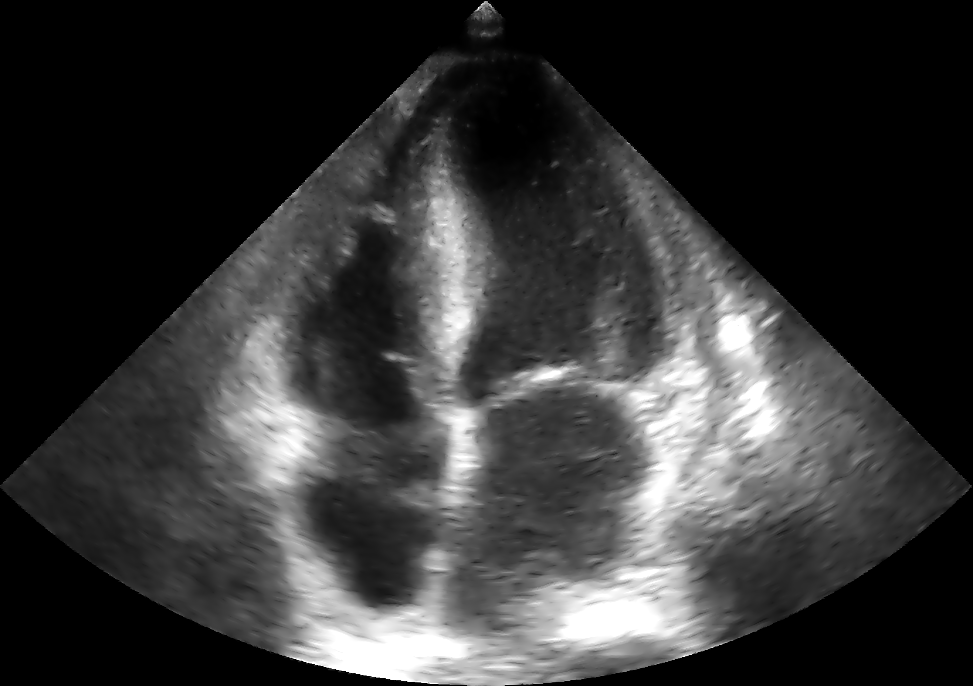
\includegraphics[width=\textwidth]{figures/cardiac3_clpdf.png}};
      \spy on (0.1, 0.2) in node [redwindow, anchor=north] at ($(figA.south)$);
    \end{tikzpicture}
    \caption{CLPD-F}
  \end{subfigure}%
  \begin{subfigure}[b]{0.15\textwidth}
    \begin{tikzpicture}[
        spy using outlines={%
          rectangle,magnification=3,size=\textwidth,
          every spy on node/.append style={redwindow}
        }
      ]
      \node (figA) at (0.0,0.0) {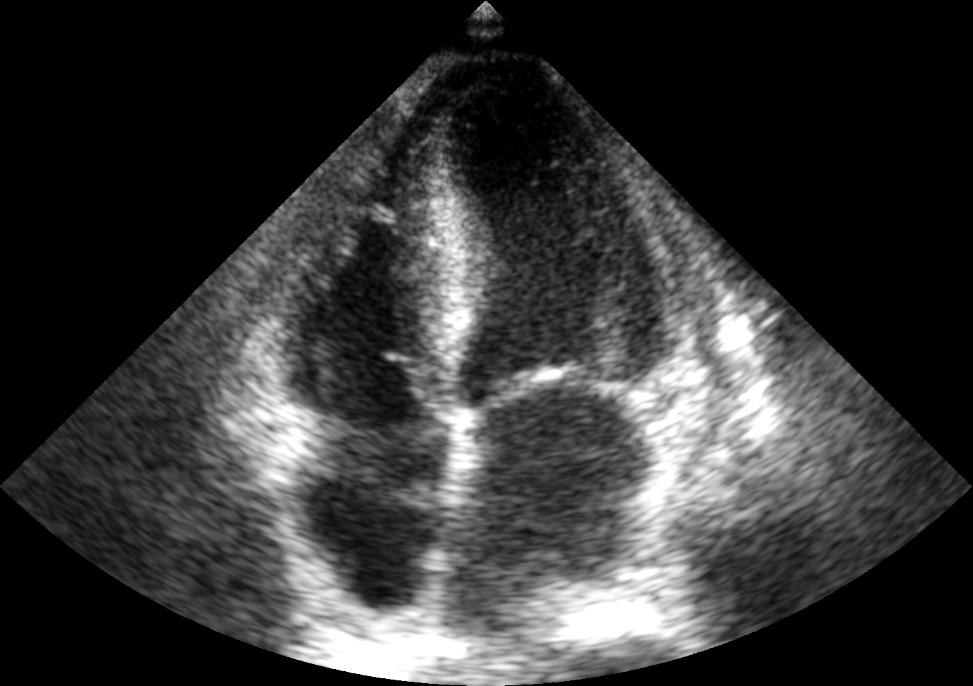
\includegraphics[width=\textwidth]{figures/cardiac3.png}};
      \spy on (0.1, 0.2) in node [redwindow, anchor=north] at ($(figA.south)$);
    \end{tikzpicture}
    \caption{Original}\label{fig:cardiac3_original}
  \end{subfigure}
  \caption{
    Results on echocardiographic 4-chamber view.
    The red squares are zooming on the left-ventricle.
  }\label{fig:cardiac3}
  \vspace{-0.15in}
\end{figure*}



\begin{figure*}
  \vspace{-0.1in}
  \centering
  \begin{subfigure}[b]{0.15\textwidth}
    \begin{tikzpicture}[
        spy using outlines={%
          rectangle,magnification=3,size=\textwidth,
          every spy on node/.append style={transparentwindow}
        }
      ]
      \node (figA) at (0.0,0.0) {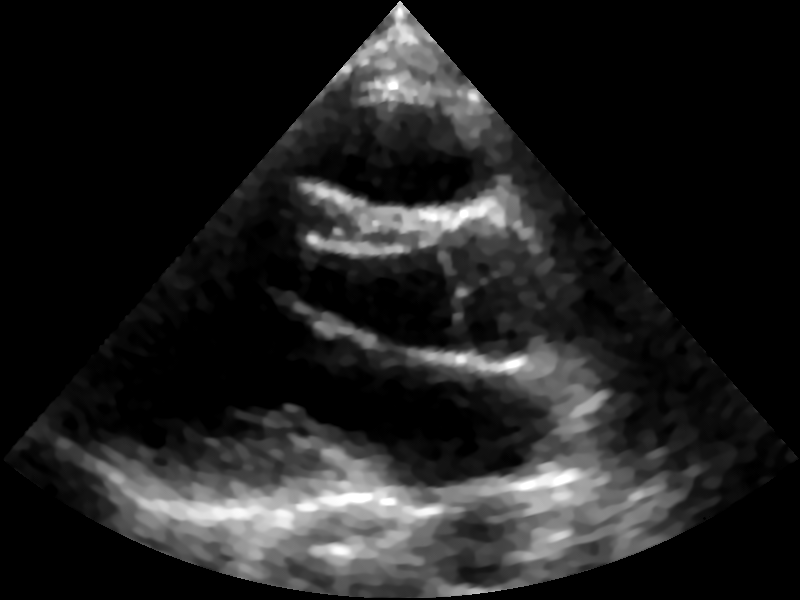
\includegraphics[width=\textwidth]{figures/cardiac1_osrad.png}};
      \spy on (0.05, 0.05) in node [redwindow, anchor=north] at ($(figA.south)$);
    \end{tikzpicture}
    \caption{OSRAD}
  \end{subfigure}%
  \begin{subfigure}[b]{0.15\textwidth}
    \begin{tikzpicture}[
        spy using outlines={%
          rectangle, magnification=3,size=\textwidth,
          every spy on node/.append style={transparentwindow}
        }
      ]
      \node (figA) at (0.0,0.0) {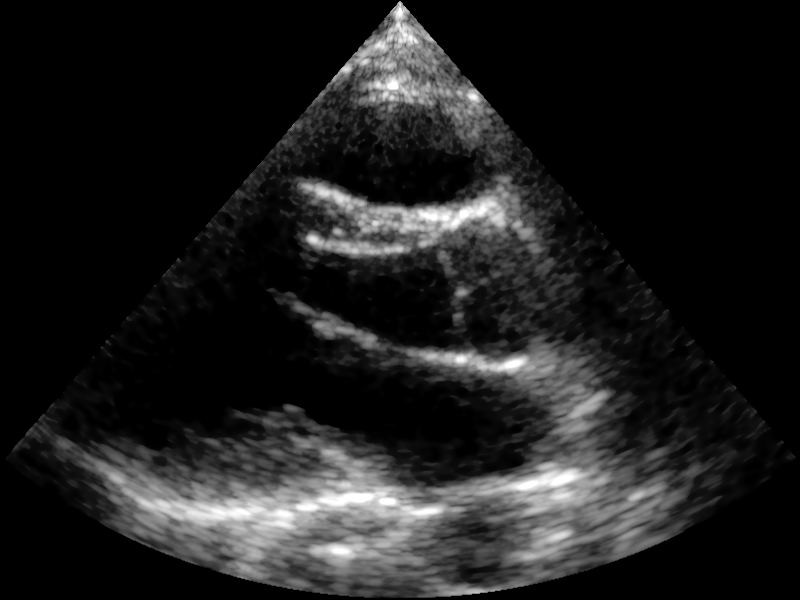
\includegraphics[width=\textwidth]{figures/cardiac1_admss.png}};
      \spy on (0.05, 0.05) in node [redwindow, anchor=north] at ($(figA.south)$);
    \end{tikzpicture}
    \caption{ADMSS}
  \end{subfigure}%
  \begin{subfigure}[b]{0.15\textwidth}
    \begin{tikzpicture}[
        spy using outlines={%
          rectangle, magnification=3,size=\textwidth,
          every spy on node/.append style={transparentwindow}
        }
      ]
      \node (figA) at (0.0,0.0) {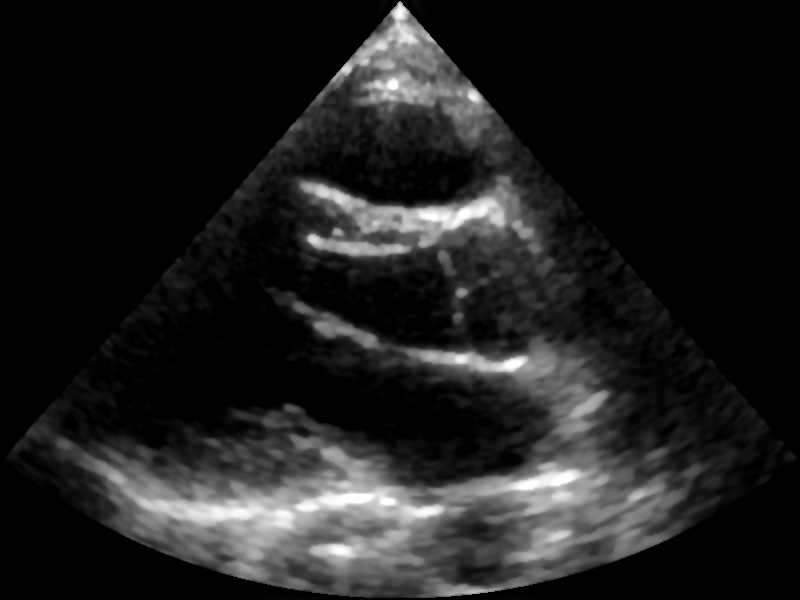
\includegraphics[width=\textwidth]{figures/cardiac1_lpndsf.png}};
      \spy on (0.05, 0.05) in node [redwindow, anchor=north] at ($(figA.south)$);
    \end{tikzpicture}
    \caption{LPNDSF}
  \end{subfigure}%
  \begin{subfigure}[b]{0.15\textwidth}
    \begin{tikzpicture}[
        spy using outlines={%
          rectangle,magnification=3,size=\textwidth,
          every spy on node/.append style={transparentwindow}
        }
      ]
      \node (figA) at (0.0,0.0) {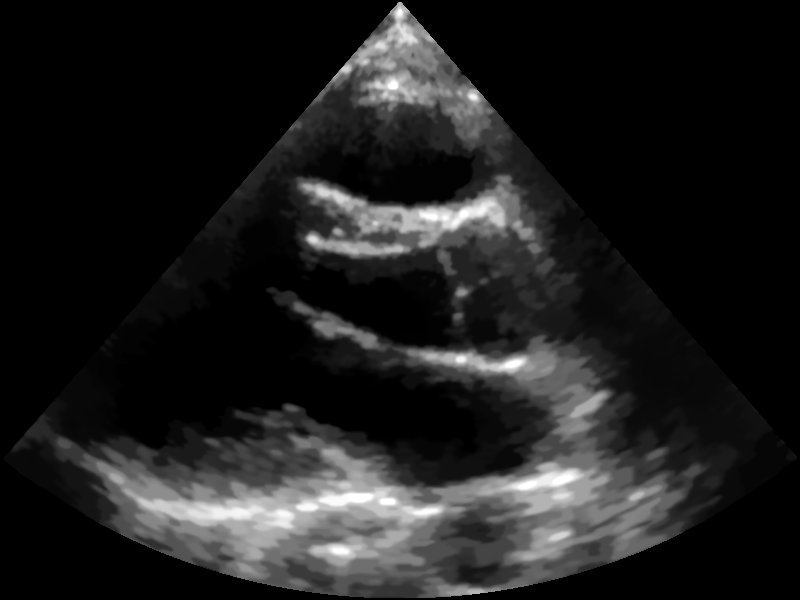
\includegraphics[width=\textwidth]{figures/cardiac1_mnlm.png}};
      \spy on (0.05, 0.05) in node [redwindow, anchor=north] at ($(figA.south)$);
    \end{tikzpicture}
    \caption{MNLM}
  \end{subfigure}%
  \begin{subfigure}[b]{0.15\textwidth}
    \begin{tikzpicture}[
        spy using outlines={%
          rectangle,magnification=3,size=\textwidth,
          every spy on node/.append style={transparentwindow}
        }
      ]
      \node (figA) at (0.0,0.0) {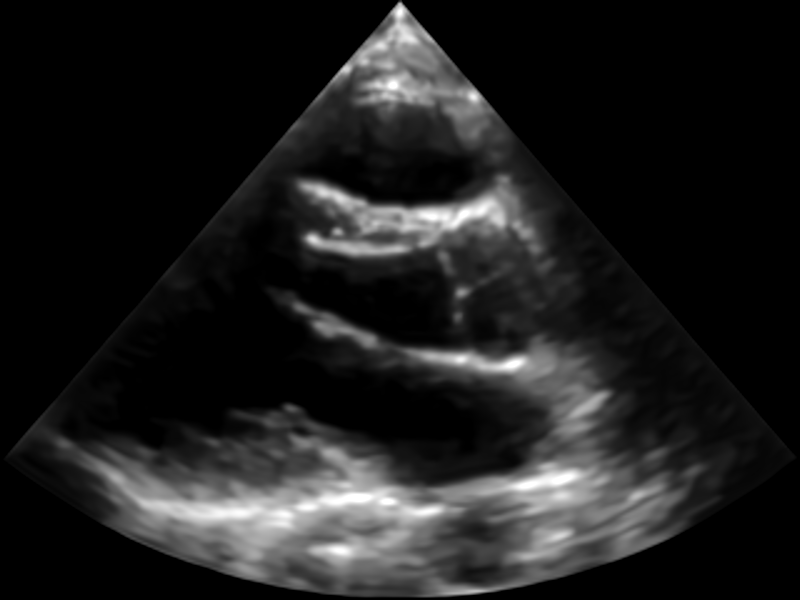
\includegraphics[width=\textwidth]{figures/cardiac1_nllr.png}};
      \spy on (0.05, 0.05) in node [redwindow, anchor=north] at ($(figA.south)$);
    \end{tikzpicture}
    \caption{NLLR}
  \end{subfigure}%
  \begin{subfigure}[b]{0.15\textwidth}
    \begin{tikzpicture}[
        spy using outlines={%
          rectangle,magnification=3,size=\textwidth,
          every spy on node/.append style={transparentwindow}
        }
      ]
      \node (figA) at (0.0,0.0) {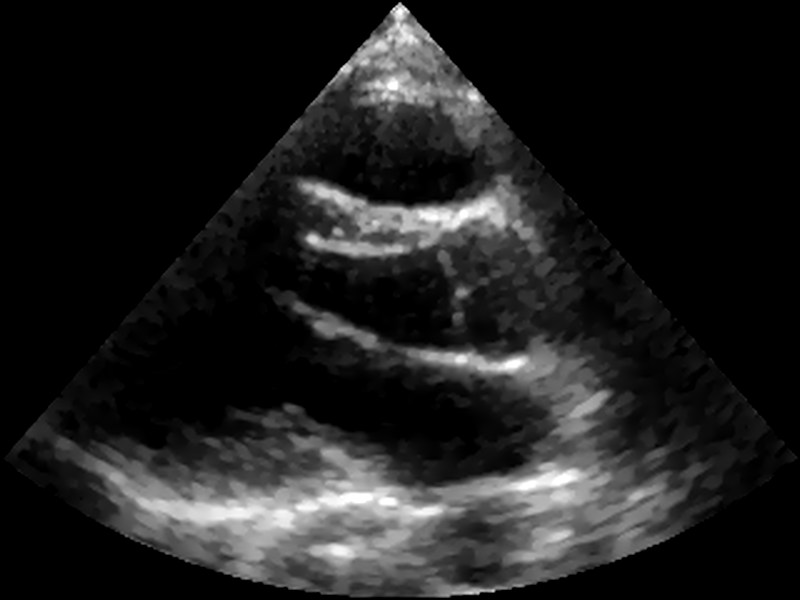
\includegraphics[width=\textwidth]{figures/cardiac1_pfdtv.png}};
      \spy on (0.05, 0.05) in node [redwindow, anchor=north] at ($(figA.south)$);
    \end{tikzpicture}
    \caption{PFDTV}
  \end{subfigure}\\
  %% \begin{subfigure}[b]{0.15\textwidth}
  %%   \begin{tikzpicture}[
  %%       spy using outlines={%
  %%         rectangle,magnification=3,size=\textwidth,
  %%         every spy on node/.append style={transparentwindow}
  %%       }
  %%     ]
  %%     \node (figA) at (0.0,0.0) {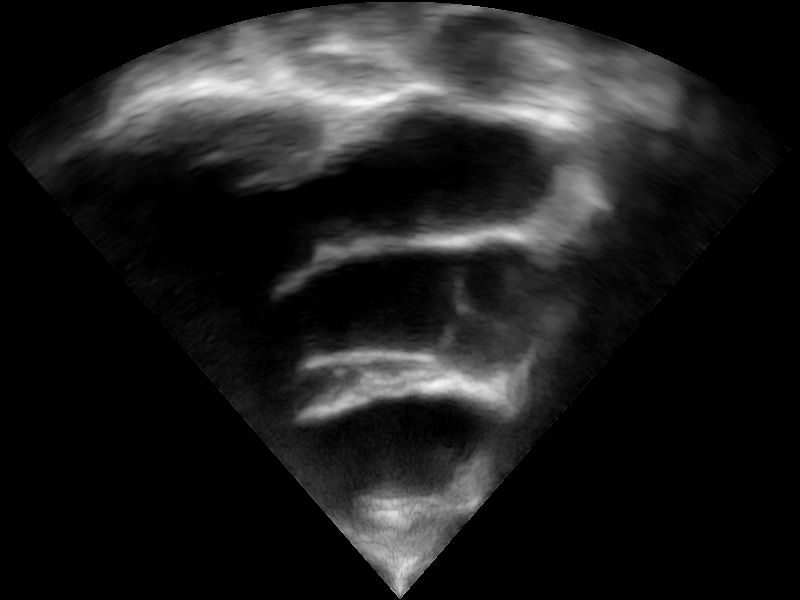
\includegraphics[width=\textwidth, trim={4cm 4cm 4cm 0cm}, clip]{figures/cardiac1_clpdQ.png}};
  %%     \spy on (0.05, 0.05) in node [redwindow, anchor=north] at ($(figA.south)$);
  %%   \end{tikzpicture}
  %%   \caption{CLPD-SSNR}
  %% \end{subfigure}%
  \begin{subfigure}[b]{0.15\textwidth}
    \begin{tikzpicture}[
        spy using outlines={%
          rectangle,magnification=3,size=\textwidth,
          every spy on node/.append style={transparentwindow}
        }
      ]
      \node (figA) at (0.0,0.0) {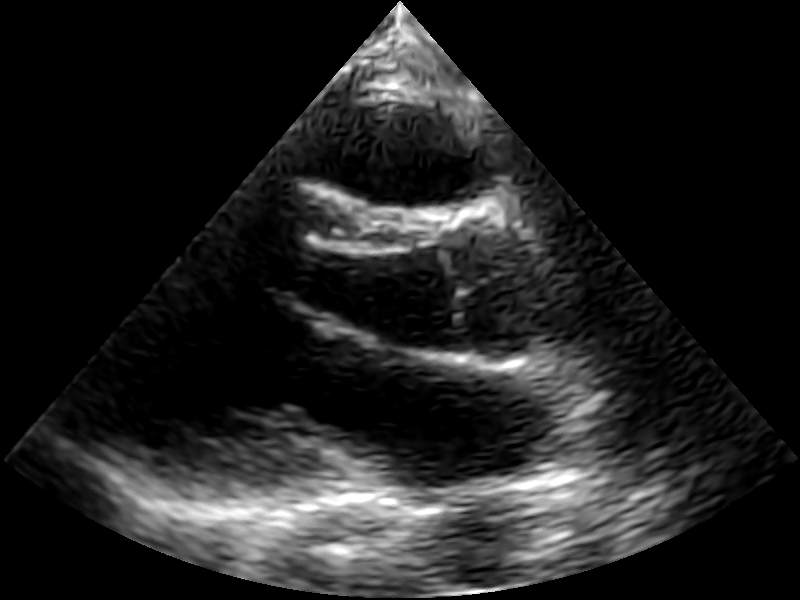
\includegraphics[width=\textwidth]{figures/cardiac1_clpda.png}};
      \spy on (0.05, 0.05) in node [redwindow, anchor=north] at ($(figA.south)$);
    \end{tikzpicture}
    \caption{CLPD-A}
  \end{subfigure}%
  \begin{subfigure}[b]{0.15\textwidth}
    \begin{tikzpicture}[
        spy using outlines={%
          rectangle,magnification=3,size=\textwidth,
          every spy on node/.append style={transparentwindow}
        }
      ]
      \node (figA) at (0.0,0.0) {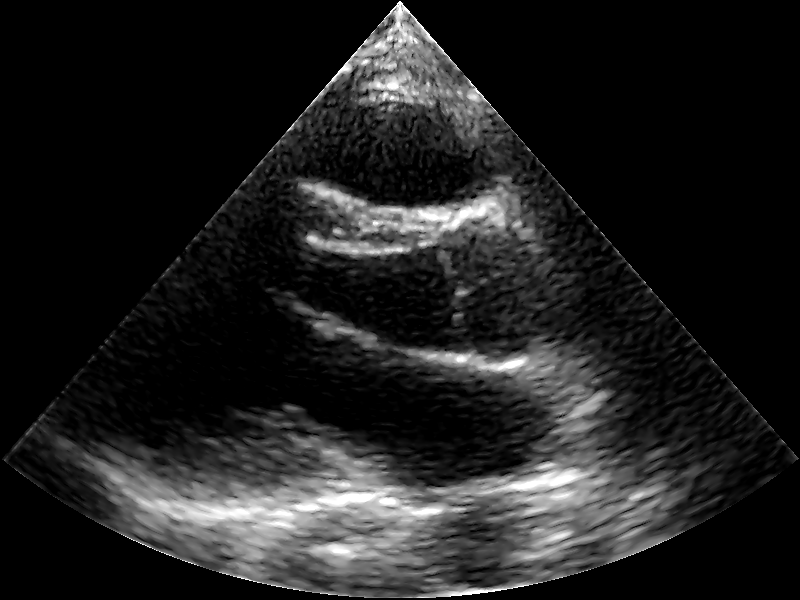
\includegraphics[width=\textwidth]{figures/cardiac1_clpdb.png}};
      \spy on (0.05, 0.05) in node [redwindow, anchor=north] at ($(figA.south)$);
    \end{tikzpicture}
    \caption{CLPD-B}
  \end{subfigure}%
  \begin{subfigure}[b]{0.15\textwidth}
    \begin{tikzpicture}[
        spy using outlines={%
          rectangle,magnification=3,size=\textwidth,
          every spy on node/.append style={transparentwindow}
        }
      ]
      \node (figA) at (0.0,0.0) {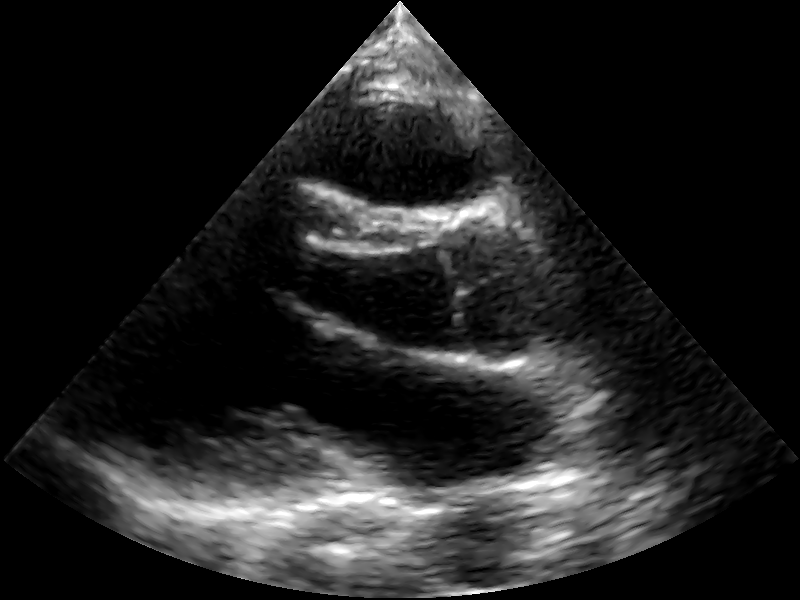
\includegraphics[width=\textwidth]{figures/cardiac1_clpdc.png}};
      \spy on (0.05, 0.05) in node [redwindow, anchor=north] at ($(figA.south)$);
    \end{tikzpicture}
    \caption{CLPD-C}
  \end{subfigure}%
  \begin{subfigure}[b]{0.15\textwidth}
    \begin{tikzpicture}[
        spy using outlines={%
          rectangle,magnification=3,size=\textwidth,
          every spy on node/.append style={transparentwindow}
        }
      ]
      \node (figA) at (0.0,0.0) {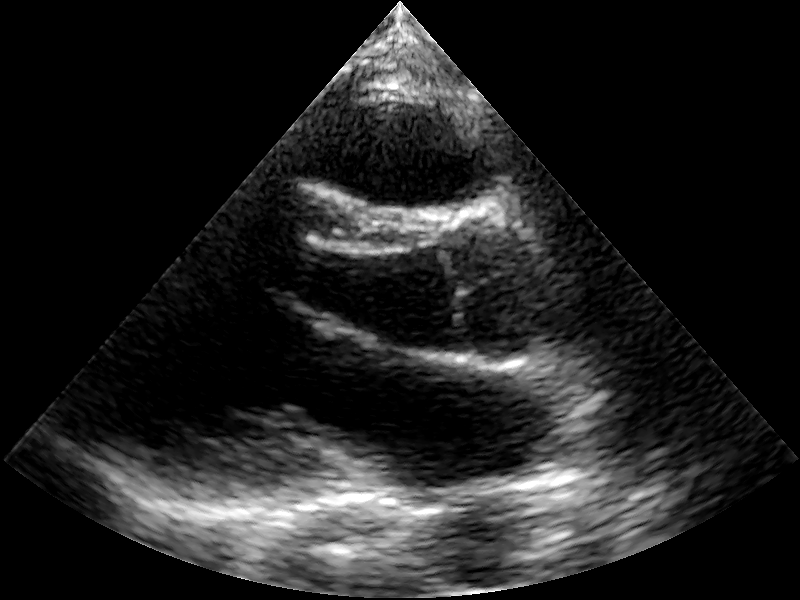
\includegraphics[width=\textwidth]{figures/cardiac1_clpdd.png}};
      \spy on (0.05, 0.05) in node [redwindow, anchor=north] at ($(figA.south)$);
    \end{tikzpicture}
    \caption{CLPD-D}
  \end{subfigure}%
  \begin{subfigure}[b]{0.15\textwidth}
    \begin{tikzpicture}[
        spy using outlines={%
          rectangle,magnification=3,size=\textwidth,
          every spy on node/.append style={redwindow}
        }
      ]
      \node (figA) at (0.0,0.0) {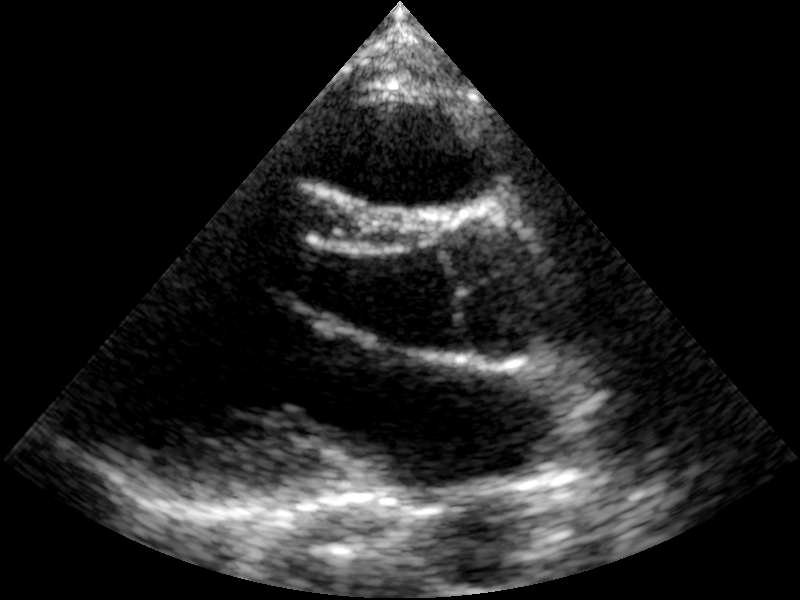
\includegraphics[width=\textwidth]{figures/cardiac1.png}};
      \spy on (0.05, 0.05) in node [redwindow, anchor=north] at ($(figA.south)$);
    \end{tikzpicture}
    \caption{Original}
  \end{subfigure}
  \caption{Results on echocardiography parasternal long-axis view.}\label{fig:cardiac1}
  \vspace{-0.1in}
\end{figure*}

%%% Local Variables:
%%% TeX-master: "master"
%%% End:


%%% Local Variables:
%%% TeX-master: "master"
%%% End:
